\chapter{Bayesian model averaging}\label{chap10}

We outline in this chapter a framework for addressing model uncertainty and averaging across different models in a probabilistically consistent manner. The discussion tackles two major computational challenges in Bayesian model averaging: the vast space of possible models and the absence of analytical solutions for the marginal likelihood.

We begin by illustrating the approach within the Gaussian linear model, assuming exogeneity of the regressors, and extend the analysis to cases with endogenous regressors, and dynamic models. Additionally, we adapt the framework to generalized linear models, including the logit, gamma, and Poisson families. Lastly, we explore alternative methods for computing marginal likelihoods, especially when the Bayesian information criterion's asymptotic approximation proves inadequate.  

Remember that we can run our GUI typing

\begin{tcolorbox}[enhanced,width=4.67in,center upper,
	fontupper=\large\bfseries,drop shadow southwest,sharp corners]
	\textit{R code. How to display our graphical user interface}
	\begin{VF}
		\begin{lstlisting}[language=R]
	shiny::runGitHub("besmarter/BSTApp", launch.browser = T)\end{lstlisting}
	\end{VF}
\end{tcolorbox} 

in the \textbf{R} package console or any \textbf{R} code editor, and once our GUI is deployed, select \textit{Bayesian Model Averaging}. However, users should see Chapter \ref{chapGUI} for other options and details.

\section{Foundation}\label{sec10_1}
Remember from Chapter \ref{chap1} that Bayesian model averaging (BMA) is an approach which takes into account model uncertainty. In particular, we consider uncertainty in the regressors (variable selection) in a regression framework where there are $K$ possible explanatory variables.\footnote{Take into account that $K$ can increase when interaction terms and/or polynomial terms of the original control variables are included.} This implies $2^K$ potential models indexed by parameters $\bm{\theta}_m$, $m=1,2,\dots,2^K$.

Following \cite{Simmons2010}, the posterior model probability is
\begin{equation*}
	\pi(\mathcal{M}_j |\bm{y})=\frac{p(\bm{y} | \mathcal{M}_j)\pi(\mathcal{M}_j)}{\sum_{m=1}^{2^K}p(\bm{y} | \mathcal{M}_m)\pi(\mathcal{M}_m)},
\end{equation*}
where $\pi(\mathcal{M}_j)$ is the prior model probability,\footnote{We attach equal prior probabilities to each model in our GUI. However, this choice gives more prior probability to the set of models of medium size (think about the $k$-th row of Pascal's triangle). An interesting alternative is to use the Beta-Binomial prior proposed by \cite{ley2009effect}.} 
\begin{equation*}
	p(\bm{y} | \mathcal{M}_j)=\int_{\bm{\Theta}_j} p(\bm{y}| \bm{\theta}_j,\mathcal{M}_j)\pi(\bm{\theta}_j | \mathcal{M}_j) d\bm{\theta}_{j}
\end{equation*}
is the marginal likelihood, and $\pi(\bm{\theta}_j | \mathcal{M}_j)$ is the prior distribution of $\bm{\theta}_j$ conditional on model $\mathcal{M}_j$.

Following \cite{Raftery93}, the posterior distribution of $\bm{\theta}$ is 
\begin{equation*}
	\pi(\bm{\theta}|\bm{y})= \sum_{m=1}^{2^K}\pi(\bm{\theta}_m|\bm{y},\mathcal{M}_m) \pi(\mathcal{M}_m|\bm{y})
\end{equation*}
The posterior distribution of the parameter vector \(\bm{\theta}\) under model \(\mathcal{M}_m\) is denoted as \(\pi(\bm{\theta}_m|\bm{y}, \mathcal{M}_m)\). The posterior mean of \(\bm{\theta}\) is given by:
\[
\mathbb{E}[\bm{\theta}|\bm{y}] = \sum_{m=1}^{2^K} \hat{\bm{\theta}}_m \, \pi(\mathcal{M}_m|\bm{y}),
\]

where \(\hat{\bm{\theta}}_m\) represents the posterior mean under model \(\mathcal{M}_m\).

The variance of the \(k\)-th element of \(\bm{\theta}\) given the data \(\bm{y}\) is:
\[
\text{Var}(\theta_{km}|\bm{y}) = \sum_{m=1}^{2^K} \pi(\mathcal{M}_m|\bm{y}) \, \widehat{\text{Var}}(\theta_{km}|\bm{y}, \mathcal{M}_m) + \sum_{m=1}^{2^K} \pi(\mathcal{M}_m|\bm{y}) \left( \hat{\theta}_{km} - \mathbb{E}[\theta_{km}|\bm{y}] \right)^2,
\]

where \(\widehat{\text{Var}}(\theta_{km}|\bm{y}, \mathcal{M}_m)\) denotes the posterior variance of the \(k\)-th element of \(\bm{\theta}\) under model \(\mathcal{M}_m\).

The posterior variance highlights how BMA accounts for model uncertainty. The first term represents the weighted variance of each model, averaged across all potential models, while the second term reflects the stability of the estimates across models. The greater the variation in estimates between models, the higher the posterior variance.

The posterior predictive distribution is
\begin{equation*}
	\pi(\bm{y}_0|\bm{y})= \sum_{m=1}^{2^K}p_m(\bm{y}_0|\bm{y},\mathcal{M}_m) \pi(M_m|\bm{y})
\end{equation*}

where $p_m(\bm{y}_0|\bm{y},\mathcal{M}_m)=\int_{\bm{\Theta}_m} p(\bm{y}_0|\bm{y},\bm{\theta}_m,\mathcal{M}_m)\pi(\bm{\theta}_m |\bm{y}, \mathcal{M}_m) d\bm{\theta}_{m}$ is the posterior predictive distribution under model $\mathcal{M}_m$. 

Another important statistic in BMA is the posterior inclusion probability associated with variable $\bm{x}_k$, $k=1,2,\dots,K$, which is

\begin{equation*}
	PIP(\bm{x}_k)=\sum_{m=1}^{2^K}\pi(\mathcal{M}_m|\bm{y})\times \mathbbm{1}_{k,m},
\end{equation*}
where
$\mathbbm{1}_{k,m}= \left\{ \begin{array}{lcc}
	1&   if  & \bm{x}_{k}\in \mathcal{M}_m \\
	\\ 0 &  if & \bm{x}_{k}\not \in \mathcal{M}_m
\end{array}
\right\}.$\\

\cite{Kass1995} suggest that posterior inclusion probabilities (PIP) less than 0.5 are evidence against the regressor, $0.5\leq PIP<0.75$ is weak evidence, $0.75\leq PIP<0.95$ is positive evidence, $0.95\leq PIP<0.99$ is strong evidence, and $PIP\geq 0.99$ is very strong evidence.

There are two main computational issues in implementing BMA based on variable selection. First, the number of models in the model space is $2^K$, which sometimes can be enormous. For instance, three regressors imply just eight models, see Table \ref{tab:chap10}, but 40 regressors implies approximately  1.1e+12 models. Take into account that models always include the intercept, and all regressors should be standardized to avoid scale issues.\footnote{Scaling variables is always an important step in variable selection.} The second computational issue is calculating the marginal likelihood $p(\bm{y} | \mathcal{M}_j)=\int_{\bm{\Theta}_j} p(\bm{y}| \bm{\theta}_j,\mathcal{M}_j)\pi(\bm{\theta}_j | \mathcal{M}_j) d\bm{\theta}_{j}$, which most of the time does not have an analytic solution. 

\begin{table}[!ht]
	\tabletitle{Space of models: Three regressors.}\label{tab:chap10}
%	\begin{threeparttable}
		\resizebox{1\textwidth}{!}{\begin{minipage}{\textwidth}
				\begin{tabular}{ccccccccc}
					 Regressor & \multicolumn{8}{c}{Inclusion}\\
					\hline
					$x_1$ & 1 & 1 & 1 & 1 & 0 & 0 & 0 & 0\\
					$x_2$ & 1 & 1 & 0 & 0 & 1 & 1 & 0 & 0\\
					$x_3$ & 1 & 0 & 1 & 0 & 1 & 0 & 1 & 0\\ 			
				\end{tabular}
				\begin{tablenotes}[para,flushleft]
					\footnotesize \textit{Notes}: ``1" indicates inclusion of the regressor, and ``0" indicates no inclusion. The space of models is composed by 8 models. The model always includes intercept.\\
				\end{tablenotes}
		\end{minipage}}
%	\end{threeparttable}
\end{table}
The first computational issue is basically a problem of ranking models. This can be tackled using different approaches, such as Occam's window criterion \cite{Madigan1994,Raftery1997}, reversible jump Markov chain Monte Carlo computation \cite{Green1995}, Markov chain Monte Carlo model composition \cite{madigan95}, and multiple testing using intrinsic priors \cite{Casella2006} or nonlocal prior densities \cite{Johnson2012}. We focus on Occam's window and Markov chain Monte Carlo model composition in our GUI.\footnote{Variable selection (model selection or regularization) is a topic related to model uncertainty. Approaches such as stochastic search variable selection (spike and slab) \cite{George1993,George1997} and Bayesian Lasso \cite{Park2008} are good examples of how to tackle this issue. See Chapter \ref{chap13}.}

In Occam's window, a model is discarded if its predictive performance is much worse than that of the best model  \cite{Madigan1994,Raftery1997}.
Thus, models not belonging to $\mathcal{M}'=\left\{\mathcal{M}_j:\frac{\max_m {\pi(\mathcal{M}_m|\bm{y})}}{\pi(\mathcal{M}_j|\bm{y})}\leq c\right\}$ should be discarded, where $c$ is chosen by the user (\cite{Madigan1994} propose $c=20$).
In addition, complicated models than are less supported by the data than simpler models are also discarded, that is, $\mathcal{M}''=\left\{\mathcal{M}_j:\exists \mathcal{M}_m\in\mathcal{M}',\mathcal{M}_m\subset \mathcal{M}_j,\frac{\pi(\mathcal{M}_m|\bm{y})}{\pi(\mathcal{M}_j|\bm{y})}>1\right\}$. Then, the set of models used in BMA is $\mathcal{M}^*=\mathcal{M}'\cap \mathcal{M}''^c\in\mathcal{M}$. \cite{Raftery1997} find that the number of models in $\mathcal{M}^*$ is normally less than 25.

However, the previous theoretical framework requires finding the model with the maximum a posteriori model probability ($\max_m {\pi(\mathcal{M}_m|\bm{y})}$), which implies calculating all possible models in $\mathcal{M}$. This is computationally burdensome. Hence, a heuristic approach is proposed by \cite{Raftery2012} based on ideas of \cite{Madigan1994}. The search strategy is based on a series of nested comparisons of ratios of posterior model probabilities. Let $\mathcal{M}_0$ be a model with one regressor less than model $\mathcal{M}_1$, then:
\begin{itemize}
	\item If $\log(\pi(\mathcal{M}_0|\bm{y})/\pi(\mathcal{M}_1|\bm{y}))>\log(O_R)$, then $\mathcal{M}_1$ is rejected and $\mathcal{M}_0$ is considered.
	\item If $\log(\pi(\mathcal{M}_0|\bm{y})/\pi(\mathcal{M}_1|\bm{y}))\leq -\log(O_L)$, then $\mathcal{M}_0$ is rejected, and $\mathcal{M}_1$ is considered.
	 \item If $\log(O_L)<\log(\pi(\mathcal{M}_0|\bm{y})/\pi(\mathcal{M}_1|\bm{y}))\leq \log(O_R$), $\mathcal{M}_0$ and $\mathcal{M}_1$ are considered.
\end{itemize} 
Here $O_R$ is a number specifying the maximum ratio for excluding models in Occam's window, and $O_L=1/O_R^{2}$ is defined by default in \cite{Raftery2012}. The search strategy can be ``up'', adding one regressor, or ``down'', dropping one regressor (see \cite{Madigan1994} for details about the down and up algorithms). The leaps and bounds algorithm \cite{Furnival1974} is implemented to improve the computational efficiency of this search strategy \cite{Raftery2012}. Once the set of potentially acceptable models is defined, we discard all the models that are not in $\mathcal{M}'$, and the models that are in $\mathcal{M}''$ where 1 is replaced by $\exp\left\{O_R\right\}$ due to the leaps and bounds algorithm giving an approximation to BIC, so as to ensure that no good models are discarded.

The second approach that we consider in our GUI to tackle the model space size issue is Markov chain Monte Carlo model composition (MC3) \cite{madigan1995bayesian1}.
In particular, given the space of models $\mathcal{M}_m$, we simulate a chain of $\mathcal{M}_s$ models, $s = 1, 2, ..., S<<2^K$, where the algorithm randomly extracts a candidate model $\mathcal{M}_c$ from a neighborhood of models ($nbd(\mathcal{M}_m)$) that consists of the actual model itself and the set of models with either one variable more or one variable less \cite{Raftery1997}. Therefore, there is a transition kernel in the space of models $q(\mathcal{M}_m\rightarrow \mathcal{M}_c)$, such that $q(\mathcal{M}_m\rightarrow \mathcal{M}_{c})=0 \ \forall \mathcal{M}_{c}\notin nbd(\mathcal{M}_m)$ and $q(\mathcal{M}_m\rightarrow \mathcal{M}_{c})=\frac{1}{|nbd(\mathcal{M}_m)|} \ \forall \mathcal{M}_m\in nbd(\mathcal{M}_m)$, $|nbd(\mathcal{M}_m)|$ being the number of neighbors of $\mathcal{M}_m$. This candidate model is accepted with probability

\begin{equation*}
	\alpha (\mathcal{M}_{s-1},\mathcal{M}_{c})=\min \bigg \{ \frac{|nbd(\mathcal{M}_m)|p(\bm{y} | \mathcal{M}_c)\pi(\mathcal{M}_c)}{|nbd(\mathcal{M}^{c})|p(\bm{y}| \mathcal{M}_{(s-1)})\pi(\mathcal{M}_{(s-1)})},1 \bigg \}.
\end{equation*}

Observe that by construction $|nbd(\mathcal{M}_m)|=|nbd(\mathcal{M}_c)|=k$, except in extreme cases where a model has only one regressor or has all regressors.

The Bayesian information criterion is a possible solution for the second computational issue in BMA, that is, calculating the marginal likelihood when there is no an analytic solution. Defining $h(\bm{\theta}|\mathcal{M}_j)=-\frac{\log(p(\bm{y}| \bm{\theta}_j,\mathcal{M}_j)\pi(\bm{\theta}_j | \mathcal{M}_j))}{N}$, then $p(\bm{y} | \mathcal{M}_j)=\int_{\bm{\Theta}_j} \exp\left\{-N h(\bm{\theta}|\mathcal{M}_j)\right\}  d\bm{\theta}_{j}$. If $N$ is sufficiently large (technically $N\to \infty$), we can make the following assumptions \cite{Hoeting1999}:

\begin{itemize}
	\item We can use the Laplace method for approximating integrals \cite{Tierney1986}.
	\item The posterior mode is reached at the same point as the maximum likelihood estimator (MLE), denoted by $\hat{\bm{\theta}}_{MLE}$.
\end{itemize}

We get the following results under these assumptions:
\begin{align*}
	p(\bm{y} | \mathcal{M}_j)\approx&\left( \frac{2\pi}{N}\right)^{K_j/2}|\bm{\Sigma}|^{-1/2} \exp\left\{-N h(\bm{\hat{\theta}}_j^{MLE}|\mathcal{M}_j)\right\}, \ N\rightarrow\infty,
\end{align*}
where $\bm{\Sigma}$ is the inverse of the Hessian matrix of $h(\bm{\hat{\theta}}_j^{MLE}|\mathcal{M}_j)$, and $K_j=dim\left\{\bm{\theta}_j\right\}$.

This implies
\begin{align*}
	\log\left(p(\bm{y} | \mathcal{M}_j)\right)\approx& \frac{K_j}{2}\log(2\pi)- \frac{K_j}{2}\log(N) -\frac{1}{2}\log(|\bm{\Sigma}|) + \log(p(\bm{y}| \bm{\hat{\theta}}_j^{MLE},\mathcal{M}_j))\\
	&+\log(\pi(\bm{\hat{\theta}}_j^{MLE} | \mathcal{M}_j)), \ N\rightarrow\infty.
\end{align*}

Since $\frac{K_j}{2}\log(2\pi)$ and $\log(\pi(\bm{\hat{\theta}}_j^{MLE} | \mathcal{M}_j))$ are constants as functions of $\bm{y}$, and $|\bm{\Sigma}|$ is bounded by a finite constant, we have
\begin{align*}
	log\left(p(\bm{y} | \mathcal{M}_j)\right)\approx& -\frac{K_j}{2}\log(N)+\log(p(\bm{y}| \bm{\hat{\theta}}_j^{MLE},\mathcal{M}_j))= -\frac{BIC}{2}, \ N \rightarrow \infty.
\end{align*}

The marginal likelihood thus asymptotically converges to a linear transformation of the Bayesian Information Criterion (BIC), significantly simplifying its calculation. In addition, the BIC is consistent, that is, the probability of uncovering the population statistical model converges to one as the sample size converges to infinity given a $\mathcal{M}$-closed view \cite[Chap.~6]{Bernardo1994}, that is, one of the models in consideration is the population statistical model (data generating process) \cite{schwarz1978estimating, burnham2004multimodel}. In case that there is an $\mathcal{M}$-completed view of nature, that is, there is a true data generating process, but the space of models that we are comparing does not include it, the BIC asymptotically selects the model that minimizes the Kullback-Leiber (KL) divergence to the true (population) model \cite[Chap. ~4]{claeskens2008model}. 

\section{The Gaussian linear model}\label{sec10_2}

The Gaussian linear model specifies $\bm{y}=\alpha\bm{i}_N+\bm{X}_m\bm{\beta}_m+\bm{\mu}_m$ such that $\bm{\mu}_m\sim{N}(\bm{0},\sigma^2\bm{I}_n)$, and $\bm{X}_m$ does not have the column of ones. Following \cite{koop2003bayesian}, the conjugate prior for the location parameters is $\bm{\beta}_m|\sigma^2 \sim {N}(\bm{\beta}_{m0}, \sigma^2 \bm{B}_{m0})$, and the priors for $\sigma^2$ and $\alpha$ can be improper, as these parameters are common to all models $\mathcal{M}_m$. Particularly, $\pi(\sigma^2)\propto 1/\sigma^2$ (Jeffreys' prior for the linear Gaussian model, see \cite{prior1991bayesian}) and $\pi(\alpha)\propto 1$.

The selection of the hyperparameters of $\bm{\beta}_m$ is more critical, as these parameters are not common to all models. A very common prior for the location parameters in the BMA literature is the Zellner's prior \cite{zellner1986assessing}, where $\bm{\beta}_{m0}=\bm{0}_m$ and $\bm{B}_{m0}=(g_m\bm{X}_m^{\top}\bm{X}_m)^{-1}$. Observe that this covariance matrix is similar to the covariance matrix of the ordinary least squares estimator of the location parameters. This suggests that there is compatibility between the prior information and the sample information, and the only parameter to elicit is $g_m\geq 0$, which facilitates the elicitation process, as eliciting covariance matrices is a very hard endeavor.

Following same steps as in Section \ref{sec43}, the posterior conditional distribution of $\bm{\beta}_m$ has covariance matrix $\sigma^2\bm{B}_{mn}$, where $\bm{B}_{mn}=((1+g_m)\bm{X}_m^{\top}\bm{X}_m)^{-1}$ (Exercise 1), which means that $g_m=0$ implies a non-informative prior, whereas $g_m=1$ implies that prior and data information have same weights. We follow \cite{fernandez2001benchmark}, who recommend
\begin{align*}
	g_m & =
	\begin{Bmatrix}
		1/K^2, & N \leq K^2\\
		1/N, & N>K^2 
	\end{Bmatrix}.
\end{align*}  
 
Given the likelihood function, 
\begin{equation*}
	p(\bm{\beta}_m, \sigma^2|\bm{y}, \bm{X}_m) = (2\pi\sigma^2)^{-\frac{N}{2}} \exp \left\{-\frac{1}{2\sigma^2} (\bm{y} - \alpha\bm{i}_N - \bm{X}_m\bm{\beta}_m)^{\top}(\bm{y} - \alpha\bm{i}_N - \bm{X}_m\bm{\beta}_m) \right\},
\end{equation*}
the marginal likelihood associated with model $\mathcal{M}_m$ is proportional to (Exercise 1) 
\begin{align*}
	p(\bm{y}|\mathcal{M}_m)&\propto \left(\frac{g_m}{1+g_m}\right)^{k_m/2} \left[(\bm{y}-\bar{y}\bm{i}_N)^{\top}(\bm{y}-\bar{y}\bm{i}_N)-\frac{1}{1+g_m}(\bm{y}^{\top}\bm{P}_{X_m}\bm{y})\right]^{-(N-1)/2},
\end{align*}
where all parameters are indexed to model $\mathcal{M}_m$, $\bm{P}_{X_m}=\bm{X}_m(\bm{X}_m^{\top}\bm{X}_m)^{-1}\bm{X}_m$ is the projection matrix on the space generated by the columns of $\bm{X}_m$, and $\bar{y}$ is the sample mean of $\bm{y}$.

We implement in our GUI four approaches to perform BMA in the Gaussian linear model: the BIC approximation using the Occam's window approach, the MC3 algorithm using the analytical expression for calculating the marginal likelihood, an instrumental variable approach based on conditional likelihoods, and dynamic variable selection.\\

\textbf{Example: Simulation exercise}

Let's perform a simulation exercise to assess the performance of the BIC approximation using the Occam's window, and the Markov chain Monte Carlo model composition approaches. Let's set a model where the computational burden is low and we know the data generating process (population statistical model). In particular, we set 10 regressors such that $x_k\sim N(1, 1)$, $k =1,\dots,6$, and $x_k\sim B(0.5)$, $k=7,\dots,10$. We set $\bm{\beta}=[1 \ 0 \ 0 \ 0 \ 0.5 \ 0, 0, 0, 0, -0.7]^{\top}$ such that just $x_1$, $x_5$ and $x_{10}$ are relevant to drive $y_i=1+\bm{x}^{\top}\bm{\beta}+\mu_i$, $\mu_i\sim N(0,0.5^2)$. Observe that we just have $2^{10}=1024$ models in this setting, thus, we can calculate the posterior model probability for each model. 

Our GUI uses the commands \textit{bicreg} and \textit{MC3.REG} from the package \textit{BMA} to perform Bayesian model averaging in the linear regression model using the BIC approximation and MC3, respectively. These commands in turn are based on \cite{Raftery1995} and \cite{Raftery1997}. The following code shows how to perform the simulation and get the posterior mean and standard deviation using these commands with the default values of hyperparameters and tuning parameters.

\begin{tcolorbox}[enhanced,width=4.67in,center upper,
	fontupper=\large\bfseries,drop shadow southwest,sharp corners]
	\textit{R code. Simulation exercise: Bayesian model averaging, small setting}
	\begin{VF}
		\begin{lstlisting}[language=R]
rm(list = ls()); set.seed(010101)
N <- 1000
K1 <- 6; K2 <- 4; K <- K1 + K2
X1 <- matrix(rnorm(N*K1,1 ,1), N, K1)
X2 <- matrix(rbinom(N*K2, 1, 0.5), N, K2)
X <- cbind(X1, X2); e <- rnorm(N, 0, 0.5)
B <- c(1,0,0,0,0.5,0,0,0,0,-0.7)
y <- 1 + X%*%B + e
BMAglm <- BMA::bicreg(X, y, strict = FALSE, OR = 50) 
summary(BMAglm)
\end{lstlisting}
	\end{VF}
\end{tcolorbox} 

\begin{tcolorbox}[enhanced,width=4.67in,center upper,
	fontupper=\large\bfseries,drop shadow southwest,sharp corners]
	\textit{R code. Simulation exercise: Bayesian model averaging, small setting}
	\begin{VF}
		\begin{lstlisting}[language=R]
BMAreg <- BMA::MC3.REG(y, X, num.its=500)
Models <- unique(BMAreg[["variables"]])
nModels <- dim(Models)[1]
nVistModels <- dim(BMAreg[["variables"]])[1]
PMP <- NULL
for(m in 1:nModels){
	idModm <- NULL
	for(j in 1:nVistModels){
		if(sum(Models[m,] == BMAreg[["variables"]][j,]) == K){
			idModm <- c(idModm, j)
		}else{
			idModm <- idModm
		} 
	}
	PMPm <- sum(BMAreg[["post.prob"]][idModm])
	PMP <- c(PMP, PMPm)
}
PIP <- NULL
for(k in 1:K){
	PIPk <- sum(PMP[which(Models[,k] == 1)])
	PIP <- c(PIP, PIPk)
}
plot(PIP)
Means <- matrix(0, nModels, K)
Vars <- matrix(0, nModels, K)
for(m in 1:nModels){
	idXs <- which(Models[m,] == 1)
	if(length(idXs) == 0){
		Regm <- lm(y ~ 1)
	}else{
		Xm <- X[, idXs]
		Regm <- lm(y ~ Xm)
		SumRegm <- summary(Regm)
		Means[m, idXs] <- SumRegm[["coefficients"]][-1,1]
		Vars[m, idXs] <- SumRegm[["coefficients"]][-1,2]^2 
	} 
}
BMAmeans <- colSums(Means*PMP)
BMAsd <- (colSums(PMP*Vars)  + colSums(PMP*(Means-matrix(rep(BMAmeans, each = nModels), nModels, K))^2))^0.5
BMAmeans
[1]  1.001771e+00 -5.322016e-05  6.635422e-06  3.721457e-07  4.976335e-01
[6] -1.271339e-04  1.000932e-08  2.107441e-05  6.578654e-06 -7.035557e-01 
BMAsd
[1] 1.527261e-02 1.353624e-03 5.936816e-04 1.163947e-04 1.566698e-02 1.987360e-03
[7] 2.778896e-05 1.270579e-03 6.997305e-04 3.093389e-02
BMAmeans/BMAsd
\end{lstlisting}
	\end{VF}
\end{tcolorbox}
We can see from the results that the BIC approximation with the Occam's window, and the MC3 algorithm perform a good job finding the relevant regressors, and their posterior BMA means are very close to the population values. We also see that the BMA results are very similar in the two approaches.

We can perform Bayesian model averaging in our GUI for linear Gaussian models using the BIC approximation and MC3 using Algorithms \ref{alg:BMAnormalBIC} and \ref{alg:BMAnormalMC3}, respectively. We ask in Exercise 2 to perform BMA using the dataset \textit{10ExportDiversificationHHI.csv} from \cite{Jetter2015}.  

\begin{algorithm}[h!]
	\caption{Bayesian model averaging in linear Gaussian models using the Bayesian information criterion}\label{alg:BMAnormalBIC}
	\begin{algorithmic}[1]  		 			
		\State Select \textit{Bayesian Model Averaging} on the top panel
		\State Select \textit{Normal data} model using the left radio button
		\State Select \textit{BIC} using the right radio button under \textbf{Which type do you want to perform?}
		\State Upload the dataset selecting first if there is header in the file, and the kind of separator in the \textit{csv} file of the dataset (comma, semicolon, or tab). Then, use the \textit{Browse} button under the \textbf{Choose File} legend
		\State Type the \textit{OR} number of the Occam's window in the box under \textbf{OR: Number between 5 and 50}, this is not necessary as by default there is 50
		\State Click the \textit{Go!} button
		\State Analyze results: After a few seconds or minutes, a table appears showing, for each regressor in the dataset, the PIP (posterior inclusion probability, \textbf{p!=0}), the BMA posterior mean (\textbf{EV}), the BMA standard deviation (\textbf{SD}), and the posterior mean for models with the highest PMP. At the bottom of the table, for the models with the largest PMP, the number of variables (\textbf{nVar}), the coefficient of determination (\textbf{r2}), the BIC, and the PMP (\textbf{post prob}) are displayed
		\State Download posterior results using the \textit{Download results using BIC}. There are two files, the first has the best models by row according to the PMP (last column) indicating with a 1 inclusion of the variable (0 indicates no inclusion), and the second file has the PIP, the BMA expected value and standard deviation for each variable in the dataset
	\end{algorithmic} 
\end{algorithm}

\begin{algorithm}[h!]
	\caption{Bayesian model averaging in linear Gaussian models using Markov chain Monte Carlo model composition}\label{alg:BMAnormalMC3}
	\begin{algorithmic}[1]  		 			
		\State Select \textit{Bayesian Model Averaging} on the top panel
		\State Select \textit{Normal data} model using the left radio button
		\State Select \textit{MC3} using the right radio button under \textbf{Which type do you want to perform?}
		\State Upload the dataset selecting first if there is header in the file, and the kind of separator in the \textit{csv} file of the dataset (comma, semicolon, or tab). Then, use the \textit{Browse} button under the \textbf{Choose File} legend
		\State Select MC3 iterations using the \textit{Range slider} under the label \textbf{MC3 iterations:}
		\State Click the \textit{Go!} button
		\State Analyze results: After a few seconds or minutes, a table appears showing, for each regressor in the dataset, the PIP (posterior inclusion probability, \textbf{p!=0}), the BMA posterior mean (\textbf{EV}), the BMA standard deviation (\textbf{SD}), and the posterior mean for models with the highest PMP. At the bottom of the table, for the models with the largest PMP, the number of variables (\textbf{nVar}), the coefficient of determination (\textbf{r2}), the BIC, and the PMP (\textbf{post prob}) are displayed
		\State Download posterior results using the \textit{Download results using BIC}. There are two files, the first has the best models by row according to the PMP (last column) indicating with a 1 inclusion of the variable (0 indicates no inclusion), and the second file has the PIP, the BMA expected value and standard deviation for each variable in the dataset
	\end{algorithmic} 
\end{algorithm}

We show in the following code how to program a MC3 algorithm from scratch to perform BMA using the setting from the previous simulation exercise. The first part of the code is the function to calculate the log marginal likelihood. This is a small simulation setting, thus we can calculate the marginal likelihood for all 1024 models, and then calculate the posterior model probability standardizing using the model with the largest log marginal likelihood. We see from the results that this model is the data generating process (population statistical model). We also find that the posterior inclusion probabilities for $x_{1}$, $x_{5}$ and $x_{10}$ are 1, whereas the PIP for the other variables are less than 0.05. 

Although BMA allows incorporating model uncertainty in a regression framework, sometimes it is desirable to select just one model. Two compelling alternatives are the model with the largest posterior model probability, and the median probability model. The latter is the model which includes every predictor that has posterior inclusion probability higher than 0.5. The first model is the best alternative for prediction in the case of a 0--1 loss function \cite{Clyde2004}, whereas the second is the best alternative when there is a quadratic loss function in prediction \cite{Barbieri2004}. In this simulation, the two criteria indicate selection of the data generating process.

We also show how to estimate the posterior mean and standard deviation based on BMA in this code. We see that the posterior means are very close to the population parameters.  

\begin{tcolorbox}[enhanced,width=4.67in,center upper,
	fontupper=\large\bfseries,drop shadow southwest,sharp corners]
	\textit{R code. Simulation exercise: Bayesian model averaging, small setting from scratch}
	\begin{VF}
		\begin{lstlisting}[language=R]
rm(list = ls()); set.seed(010101)
N <- 1000; K1 <- 6; K2 <- 4; K <- K1 + K2
X1 <- matrix(rnorm(N*K1,1 ,1), N, K1)
X2 <- matrix(rbinom(N*K2, 1, 0.5), N, K2)
X <- cbind(X1, X2); e <- rnorm(N, 0, 0.5)
B <- c(1,0,0,0,0.5,0,0,0,0,-0.7); y <- 1 + X%*%B + e			
LogMLfunt <- function(Model){
	indr <- Model == 1
	kr <- sum(indr)
	if(kr > 0){
		gr <- ifelse(N > kr^2, 1/N, kr^(-2))
		Xr <- matrix(Xnew[ , indr], ncol = kr)
		PX <- Xr%*%solve(t(Xr)%*%Xr)%*%t(Xr)
		s2pos <- c((t(y - mean(y))%*%(y - mean(y))) - t(y)%*%PX%*%y/(1 + gr))
		mllMod <- (kr/2)*log(gr/(1+gr))-(N-1)/2*log(s2pos)
	}else{
		gr <- ifelse(N > kr^2, 1/N, kr^(-2))
		s2pos <- c((t(y - mean(y))%*%(y - mean(y))))
		mllMod <- (kr/2)*log(gr/(1+gr))-(N-1)/2*log(s2pos)
	}
	return(mllMod)
}
combs <- expand.grid(c(0,1), c(0,1), c(0,1), c(0,1), c(0,1),c(0,1), c(0,1), c(0,1), c(0,1), c(0,1))
Xnew <- apply(X, 2, scale)
mll <- sapply(1:2^K, function(s){LogMLfunt(matrix(combs[s,], 1, K))})
MaxPMP <- which.max(mll); StMarLik <- exp(mll-max(mll))
PMP <- StMarLik/sum(StMarLik)
PMP[MaxPMP]; combs[MaxPMP,]
PIP <- NULL
for(k in 1:K){
	PIPk <- sum(PMP[which(combs[,k] == 1)]); PIP <- c(PIP, PIPk)
}
PIP
nModels <- dim(combs)[1]; Means <- matrix(0, nModels, K)
Vars <- matrix(0, nModels, K)
for(m in 1:nModels){
	idXs <- which(combs[m,] == 1)
	if(length(idXs) == 0){
		Regm <- lm(y ~ 1)
	}else{
		Xm <- X[, idXs]; Regm <- lm(y ~ Xm)
		SumRegm <- summary(Regm)
		Means[m, idXs] <- SumRegm[["coefficients"]][-1,1]
		Vars[m, idXs] <- SumRegm[["coefficients"]][-1,2]^2 
	}
}
BMAmeans <- colSums(Means*PMP)
BMAsd <- (colSums(PMP*Vars)  + colSums(PMP*(Means-matrix(rep(BMAmeans, each = nModels), nModels, K))^2))^0.5
\end{lstlisting}
	\end{VF}
\end{tcolorbox} 

The following part of the code demonstrates how to perform the MC3 algorithm. While this algorithm is not strictly necessary for this small-dimensional problem, it serves as a useful pedagogical exercise. The starting point is to set $S=100$ random models and order their log marginal likelihoods. The logic of the algorithm is to select the worst model among the $S$ models and propose a candidate model to compete against it. We repeat this process for 1000 iterations (as shown in the code). Note that 1000 iterations is fewer than the number of potential models (1024). This is the essence of the MC3 algorithm: performing fewer iterations than the number of models in the space.\footnote{Note that we have split the \textit{while} loop in the code into two pages.}

In our algorithm, we analyze all model scenarios using different conditionals and reasonably assume the same prior model probability for all models, with the same cardinality for both the actual and candidate models. The posterior model probability (PMP) can be calculated in several ways. One method is to recover the unique models from the final set of $S$ models, calculate the log marginal likelihood for these models, and then standardize by the best model among them. Another method involves calculating the PMP using the complete set of $S$ final models, accounting for the fact that some models may appear multiple times in the set, which requires summing the PMPs of repeated models. A third method is to calculate the PMP based on the relative frequency with which a model appears in the final set of $S$ models. These three methods can yield different PMPs, particularly when the number of MC3 iterations is small. In our example, using 1000 MC3 iterations, the data-generating process receives the highest PMP across all three methods.

A noteworthy aspect of this algorithm is that we can obtain a single model after significantly increasing the number of iterations (for example, try using 10,000 iterations). This can be advantageous if we require only one model. However, this approach neglects model uncertainty, which could be a desirable characteristic in some cases. As a challenge, we suggest programming an algorithm that yields $S$ different models after completing the MC3 iterations (Exercise 3).

\begin{tcolorbox}[enhanced,width=4.67in,center upper,
	fontupper=\large\bfseries,drop shadow southwest,sharp corners]
	\textit{R code. Simulation exercise: Bayesian model averaging, small setting from scratch}
	\begin{VF}
		\begin{lstlisting}[language=R]
M <- 100
Models <- matrix(rbinom(K*M, 1, p = 0.5), ncol=K, nrow = M)
mllnew <- sapply(1:M,function(s){LogMLfunt(matrix(Models[s,], 1, K))})
oind <- order(mllnew, decreasing = TRUE)
mllnew <- mllnew[oind]; Models <- Models[oind, ]; iter <- 1000
pb <- winProgressBar(title = "progress bar", min = 0, max = iter, width = 300); s <- 1
while(s <= iter){
	ActModel <- Models[M,]; idK <- which(ActModel == 1)
	Kact <- length(idK)
	if(Kact < K & Kact > 1){
		CardMol <- K; opt <- sample(1:3, 1)
		if(opt == 1){ # Same
			CandModel <- ActModel
		}else{
			if(opt == 2){ # Add
				All <- 1:K; NewX <- sample(All[-idK], 1)
				CandModel <- ActModel; CandModel[NewX] <- 1
			}else{ # Subtract
				LessX <- sample(idK, 1); CandModel <- ActModel
				CandModel[LessX] <- 0
			}
		}
	}else{
		CardMol <- K + 1
		if(Kact == K){
			opt <- sample(1:2, 1)
			if(opt == 1){ # Same
				CandModel <- ActModel
			}else{ # Subtract
				LessX <- sample(1:K, 1); CandModel <- ActModel
				CandModel[LessX] <- 0
			}
		}else{
			if(K == 1){
				opt <- sample(1:3, 1)
				if(opt == 1){ # Same
					CandModel <- ActModel
				}else{
					if(opt == 2){ # Add
						All <- 1:K; NewX <- sample(All[-idK], 1)
						CandModel <- ActModel; CandModel[NewX] <- 1
					}else{ # Subtract
						LessX <- sample(idK, 1); CandModel <- ActModel
						CandModel[LessX] <- 0
					}
				}
			}else{ # Add
				NewX <- sample(1:K, 1); CandModel <- ActModel
				CandModel[NewX] <- 1
			}
		}
	}
\end{lstlisting}
	\end{VF}
\end{tcolorbox} 

\begin{tcolorbox}[enhanced,width=4.67in,center upper,
	fontupper=\large\bfseries,drop shadow southwest,sharp corners]
	\textit{R code. Simulation exercise: Bayesian model averaging, small setting from scratch}
	\begin{VF}
		\begin{lstlisting}[language=R]
	LogMLact <- LogMLfunt(matrix(ActModel, 1, K))
	LogMLcand <- LogMLfunt(matrix(CandModel, 1, K))
	alpha <- min(1, exp(LogMLcand-LogMLact))
	u <- runif(1)
	if(u <= alpha){
		mllnew[M] <- LogMLcand; Models[M, ] <- CandModel
		oind <- order(mllnew, decreasing = TRUE)
		mllnew <- mllnew[oind]; Models <- Models[oind, ]
	}else{
		mllnew <- mllnew; Models <- Models
	}
	s <- s + 1
	setWinProgressBar(pb, s, title=paste( round(s/iter*100, 0),"% done"))
}
close(pb)
ModelsUni <- unique(Models)
mllnewUni <- sapply(1:dim(ModelsUni)[1], function(s){LogMLfunt(matrix(ModelsUni[s,], 1, K))})
StMarLik <- exp(mllnewUni-mllnewUni[1])
PMP <- StMarLik/sum(StMarLik) # PMP based on unique selected models
nModels <- dim(ModelsUni)[1]
StMarLik <- exp(mllnew-mllnew[1])
PMPold <- StMarLik/sum(StMarLik) # PMP all selected models
PMPot <- NULL
PMPap <- NULL
FreqMod <- NULL
for(m in 1:nModels){
	idModm <- NULL
	for(j in 1:M){
		if(sum(ModelsUni[m,] == Models[j,]) == K){
			idModm <- c(idModm, j)
		}else{
			idModm <- idModm
		}
	}
	PMPm <- sum(PMPold[idModm]) # PMP unique models using sum of all selected models
	PMPot <- c(PMPot, PMPm)
	PMPapm <- length(idModm)/M # PMP using relative frequency in all selected models
	PMPap <- c(PMPap, PMPapm)
	FreqMod <- c(FreqMod, length(idModm))
}
\end{lstlisting}
	\end{VF}
\end{tcolorbox} 
 
\begin{tcolorbox}[enhanced,width=4.67in,center upper,
	fontupper=\large\bfseries,drop shadow southwest,sharp corners]
	\textit{R code. Simulation exercise: Bayesian model averaging, small setting from scratch}
	\begin{VF}
		\begin{lstlisting}[language=R]
PIP <- NULL
for(k in 1:K){
	PIPk <- sum(PMP[which(ModelsUni[,k] == 1)])
	PIP <- c(PIP, PIPk)
}
Means <- matrix(0, nModels, K)
Vars <- matrix(0, nModels, K)
for(m in 1:nModels){
	idXs <- which(ModelsUni[m,] == 1)
	if(length(idXs) == 0){
		Regm <- lm(y ~ 1)
	}else{
		Xm <- X[, idXs]
		Regm <- lm(y ~ Xm)
		SumRegm <- summary(Regm)
		Means[m, idXs] <- SumRegm[["coefficients"]][-1,1]
		Vars[m, idXs] <- SumRegm[["coefficients"]][-1,2]^2 
	}
}
BMAmeans <- colSums(Means*PMP)
BMAsd <- (colSums(PMP*Vars)  + colSums(PMP*(Means-matrix(rep(BMAmeans, each = nModels), nModels, K))^2))^0.5 
\end{lstlisting}
\end{VF}
\end{tcolorbox} 

An important issue to account for regressors (model) uncertainty in the identification of causal effects, rather than finding good predictors (association relationships), is endogeneity. Thus, we also implement the instrumental variable approach of Section \ref{sec73} to tackle this issue in BMA. We assume that $\bm{\gamma}\sim {N}(\bm{0},\bm{I})$, $\bm{\beta}\sim {N}(\bm{0},\bm{I})$, and $\bm{\Sigma}^{-1} \sim {W}(3,\bm{I})$ \cite{Karl2012}.

\cite{Lenkoski2013} propose an algorithm based on conditional Bayes factors \cite{Dickey1978} that allows embedding MC3 within a Gibbs sampling algorithm. Given the candidate ($M_{c}^{2nd}$) and actual ($M_{s-1}^{2nd}$) models for the iteration $s$ in the second stage, the conditional Bayes factor is 
\begin{equation*}
	CBF^{2nd}=\frac{p(\bm{y}|M_{c}^{2nd},\bm{\gamma},\bm{\Sigma})}{p(\bm{y}|M_{s-1}^{2nd},\bm{\gamma},\bm{\Sigma})},
\end{equation*}
where 
\begin{align*}
	p(\bm{y}|M_{c}^{2nd},\bm{\gamma},\bm{\Sigma})&=\int_{\mathcal{M}^{2nd}}p(\bm{y}|\bm{\beta},\bm{\gamma},\bm{\Sigma})\pi(\bm{\beta}|M_{c}^{2nd})d\bm{\beta}\\
	&\propto |\bm{B}_n|^{-1/2} \exp\left\{\frac{1}{2}{\bm{\beta}_n}^{\top}\bm{B}_n^{-1}\bm{\beta}_n\right\}
	.
\end{align*}

In the first stage,
\begin{equation*}
	CBF^{1st}=\frac{p(\bm{y}|M_{c}^{1st},\bm{\beta},\bm{\Sigma})}{p(\bm{y}|M_{s-1}^{1st},\bm{\beta},\bm{\Sigma})},
\end{equation*}
where \begin{align*}
	p(\bm{y}|M_{c}^{1st},\bm{\beta},\bm{\Sigma})&=\int_{\mathcal{M}^{1st}}p(\bm{y}|\bm{\gamma},\bm{\beta},\bm{\Sigma})\pi(\bm{\gamma}|M_{c}^{1st})d\bm{\gamma}\\
	&\propto |\bm{G}_n|^{-1/2} \exp\left\{\frac{1}{2}{\bm{\gamma}_n}^{\top}\bm{G}_n^{-1}\bm{\gamma}_n\right\}.
\end{align*}
These conditional Bayes factors assume $\pi(M^{1st},M^{2sd})\propto 1$. See \cite{Lenkoski2013} for more details of the instrumental variable BMA algorithm.\footnote{\cite{Koop12} and \cite{Lenkoski2014} propose other frameworks for BMA taking into account endogeneity.}

\begin{algorithm}[h!]
	\caption{Instrumental variable Bayesian model averaging in linear Gaussian models}\label{alg:BMAIV}
	\begin{algorithmic}[1]  		 			
		\State Select \textit{Bayesian Model Averaging} on the top panel
		\State Select \textit{Normal data} model using the left radio button
		\State Select \textit{Instrumental variable} using the right radio button under \textbf{Which type do you want to perform?}
		\State Upload the dataset containing the dependent variable, endogenous regressors, and exogenous regressors including the constant (see Section \ref{secGUI6} for details).  User should select first if there is header in the file, and the kind of separator in the \textit{csv} file of the dataset (comma, semicolon, or tab). Then, use the \textit{Browse} button under the \textbf{Choose File} legend
		\State Upload the dataset containing the instruments (see Section \ref{secGUI6} for details).  User should select first if there is header in the file, and the kind of separator in the \textit{csv} file of the dataset (comma, semicolon, or tab). Then, use the \textit{Browse} button under the \textbf{Choose File (Instruments)} legend
		\State Write down the number of endogenous regressors in the box labeled \textbf{Number of Endogenous variables}
		\State Select MCMC iterations and burn-in using the \textit{Range slider} under the labels \textbf{MCMC iterations:} and \textbf{Burn-in Sample:}
		\State Click the \textit{Go!} button
		\State Analyze results: After a few seconds or minutes, two tables appear showing, for each regressor in the dataset, the PIP (posterior inclusion probability, \textbf{p!=0}), and the BMA posterior mean (\textbf{EV}). The top table shows the results of the second stage (main equation), and the bottom table shows the results of the first stage (auxiliary equations)
		\State Download posterior results using the \textit{Download results using IV}. There are three files, the first file has the posterior inclusion probabilities of each variable, and the BMA posterior means of the coefficients in the first stage equations, the second file shows these results for the second stage (main equation), and the third file has the posteriors chains of all parameters by iteration. 
	\end{algorithmic} 
\end{algorithm}

We perform instrumental variable BMA in our GUI using the package \textit{ivbma}. The Algorithm \ref{alg:BMAIV} shows how to perform this in our GUI. 

\clearpage

Let's perform a simulation exercise to assess the performance of the instrumental variable BMA to uncover the data generating process in presence of endogeneity.\\

\textbf{Example: Simulation exercise}

Let's assume that $y_i = 2 + 0.5x_{i1} - x_{i2} + x_{i3} + \mu_i$, where $x_{i1} = 4z_{i1} - z_{i2} + 2z_{i3} + \epsilon_{i1}$ and $x_{i2} = -2z_{i1} + 3z_{i2} - z_{i3} + \epsilon_{i2}$, such that $[\epsilon_{i1} \ \epsilon_{i2} \ \mu_i]^{\top} \sim N(\bm{0}, \bm{\Sigma})$, where $\bm{\Sigma} = \begin{bmatrix} 1 & 0 & 0.8 \\ 0 & 1 & 0.5 \\ 0.8 & 0.5 & 1 \end{bmatrix}$, for $i = 1, 2, \dots, 1000$. The endogeneity arises due to the correlation between $\mu_i$ and $x_{i1}$ and $x_{i2}$ through the stochastic errors. In addition, there are three instruments, $z_{il} \sim U(0,1)$, for $l = 1, 2, 3$, and another 18 regressors believed to influence $y_i$, which are distributed according to a standard normal distribution.

The following code shows how to perform IV BMA using the \textit{ivbma} package. We see from the results that the PIP of $x_{i1}$, $x_{i2}$, intercept and $x_{i3}$ are equal to 1, whereas the remaining PIP are close to 0. In addition, the BMA means are also close to the population values. The PIP of the first stage equations, as well as their BMA posterior means, are very close to the populations values. The same happens with the covariance matrix. 

We ask in Exercise 4 to perform BMA based on the BIC approximation and MC3 in this simulation setting. In addition, we ask in Exercise 5 to use the datasets \textit{11ExportDiversificationHHI.csv} and \textit{12ExportDiversificationHHIInstr.csv} to perform IV BMA assuming that the log of per capita gross domestic product is endogenous (\textit{avglgdpcap}). See \cite{Jetter2015} for details.     

\begin{tcolorbox}[enhanced,width=4.67in,center upper,
	fontupper=\large\bfseries,drop shadow southwest,sharp corners]
	\textit{R code. Simulation exercise: Instrumental variable Bayesian model averaging}
	\begin{VF}
		\begin{lstlisting}[language=R]
rm(list = ls())
set.seed(010101)
simIV <- function(delta1,delta2,beta0,betas1,betas2,beta2,Sigma,n,z) {
	eps <- matrix(rnorm(3*n),ncol=3) %*% chol(Sigma)
	xs1 <- z%*%delta1 + eps[,1]
	xs2 <- z%*%delta2 + eps[,2]
	x2 <- rnorm(dim(z)[1])
	y <- beta0+betas1*xs1+betas2*xs2+beta2*x2 + eps[,3]
	X <- as.matrix(cbind(xs1,xs2,1,x2)) 
	colnames(X) <- c("x1en","x2en","cte","xex")
	y <- matrix(y,dim(z)[1],1)
	colnames(y) <- c("y")
	list(X=X,y=y)
}
n <- 1000 ; p <- 3 
z <- matrix(runif(n*p),ncol=p)
rho31 <- 0.8; rho32 <- 0.5;
Sigma <- matrix(c(1,0,rho31,0,1,rho32,rho31,rho32,1),ncol=3)
delta1 <- c(4,-1,2); delta2 <- c(-2,3,-1); betas1 <- .5; betas2 <- -1; beta2 <- 1; beta0 <- 2
simiv <- simIV(delta1,delta2,beta0,betas1,betas2,beta2,Sigma,n,z)
nW <- 18
W <- matrix(rnorm(nW*dim(z)[1]),dim(z)[1],nW)
YXW<-cbind(simiv$y, simiv$X, W)
y <- YXW[,1]; X <- YXW[,2:3]; W <- YXW[,-c(1:3)]
S <- 10000; burnin <- 1000
regivBMA <- ivbma::ivbma(Y = y, X = X, Z = z, W = W, s = S+burnin, b = burnin, odens = S, print.every = round(S/10), run.diagnostics = FALSE)
PIPmain <- regivBMA[["L.bar"]] # PIP outcome
PIPmain
1.0000 1.0000 1.0000 1.0000 0.0125 0.0382 0.0145 0.0148 0.0136 0.0102 0.0070 0.0527 0.0014 0.0077 0.0211 0.0081 0.0047 0.0141 0.0028 0.0063 0.0072 0.0220
EVmain <- regivBMA[["rho.bar"]] # Posterior mean outcome
EVmain
5.105361e-01 -9.828459e-01  1.996885e+00  1.005497e+00 -1.700857e-04  9.946613e-04  1.086717e-04 -1.448951e-04  1.532812e-04  1.356334e-04 -6.027285e-05  9.119699e-04 -1.581408e-05  1.050517e-04 2.488002e-04 -6.229493e-05  4.292825e-05  3.371366e-05  5.345760e-06  5.933764e-05 5.066236e-05 1.516718e-04
PIPaux <- regivBMA[["M.bar"]] # PIP auxiliary
EVaux <- regivBMA[["lambda.bar"]] # Posterior mean auxiliary
plot(EVaux[,1])
plot(EVaux[,2])
EVsigma <- regivBMA[["Sigma.bar"]] # Posterior mean variance matrix
\end{lstlisting}
\end{VF}
\end{tcolorbox}

Bayesian model averaging has been also extended to state-space models. The point of departure is the univariate random walk state-space model (see Equations \ref{eq1Obs} and \ref{eq1St} in Chapter \ref{chap8}) conditional on model $\mathcal{M}_m$, $m=1,2\dots,M$. 
\begin{align}
	y_t&=\bm{x}_{mt}^{\top}\bm{\beta}_{mt}+\mu_{mt}\\
	\bm{\beta}_{mt}&=\bm{\beta}_{mt-1}+\bm{w}_{mt},
\end{align}
where $\mu_{mt}\sim N(0,\sigma^2)$ and $\bm{w}_{mt}\sim N(\bm{0},\bm{\Omega}_{mt})$.

Given $\bm{\beta}_{mt-1}|\bm{y}_{1:t-1}\sim N(\bm{b}_{mt-1},\bm{B}_{mt-1})$, then, we know from Chapter \ref{chap8} that $\bm{\beta}_{mt}|\bm{y}_{1:t-1}\sim N(\bm{b}_{mt-1}, \bm{R}_{mt})$, $\bm{R}_{mt}=\bm{B}_{mt-1}+\bm{\Omega}_{mt}$. 

Specification of $\bm{\Omega}_t$ can be highly demanding. Thus, a common approach is to express $\bm{\Omega}_{mt}=\frac{1-\lambda}{\lambda}\bm{B}_{mt-1}$, where $\lambda$ is called the \textit{forgetting parameter} or \textit{discount factor}, because it discounts the matrix $\bm{B}_{mt-1}$ that we would have with a deterministic state evolution into the matrix $\bm{R}_{mt}$ \cite[Chap.~4]{petris2009dynamic}. This parameter is typically slightly below 1, and implies that $\bm{R}_{mt}=\lambda^{-1}\bm{B}_{mt-1}$. ($\lambda^{-1}>1$).

\cite{raftery2010online} assume that the model changes infrequently, and its evolution is given by the transition matrix $\bm{T}=[t_{ml}]$, where $t_{ml}=P(\mathcal{M}_t=\mathcal{M}_m|\mathcal{M}_{t-1}=\mathcal{M}_l)$.

Then, the aim is to calculate the filtering distribution $p(\bm{\beta}_{mt},\mathcal{M}_t|y_t)=\sum_{m=1}^Mp(\bm{\beta}_{mt}|\mathcal{M}_t=\mathcal{M}_m,y_t)p(\mathcal{M}_t=\mathcal{M}_m|y_t)$. Thus, given the conditional distribution of the state at time $t-1$, $p(\bm{\beta}_{mt-1},\mathcal{M}_{t-1}|{y}_{t-1})=\sum_{m=1}^Mp(\bm{\beta}_{mt-1}|\mathcal{M}_{t-1}=\mathcal{M}_m,{y}_{t-1})p(\mathcal{M}_{t-1}=\mathcal{M}_m|{y}_{t-1})$, where the conditional distribution of $\bm{\beta}_{mt-1}$ is approximated by a Gaussian distribution, $\bm{\beta}_{mt-1}|\mathcal{M}_{t-1}=\mathcal{M}_{m},y_{t-1}\sim N(\bm{b}_{mt-1},\bm{B}_{mt-1})$, then the first step to get the one-step-ahead predictive distribution is getting the prediction of the model indicator, 
\begin{align*}
	p(\mathcal{M}_t=\mathcal{M}_l|y_{t-1})&=\sum_{m=1}^M p(\mathcal{M}_{t-1}=\mathcal{M}_m|y_{t-1})\times t_{lm}\\
	&\approx \frac{p(\mathcal{M}_{t-1}=\mathcal{M}_l|y_{t-1})^{\delta}+c}{\sum_{m=1}^M p(\mathcal{M}_{t-1}=\mathcal{M}_m|y_{t-1})^{\delta}+c},  
\end{align*}
where the second equality is used to avoid dealing with the $M^2$ elements of the transition matrix $\bm{T}$ such that the forgetting parameter $\delta$ is used, this parameter is slightly less than 1, and $c=0.001/M$ is introduced to handle a model probability being brought to computational zero by outliers.

Then, we get the one-step-ahead predictive distribution of the state vector, $\bm{\beta}_{mt}|\mathcal{M}_{t}=\mathcal{M}_{m},y_{t-1}\sim N(\bm{b}_{mt-1},\lambda^{-1}\bm{B}_{mt-1})$ 

Now, we consider the filtering stage, where the model filtering equation is 
\begin{align*}
	p(\mathcal{M}_t=\mathcal{M}_l|y_{t})=\frac{p(\mathcal{M}_t=\mathcal{M}_l|y_{t-1})p_l(y_t|y_{t-1})}{\sum_{m=1}^M p(\mathcal{M}_t=\mathcal{M}_m|y_{t-1})p_m(y_t|y_{t-1})},
\end{align*}
where $p_m(y_t|y_{t-1})$ is the one-step-ahead predictive distribution of $y_t|{y}_{t-1}$, which is $N(f_t,Q_t)$, where $f_t=\bm{x}_t^{\top}\bm{b}_{t-1}$ and $Q_t=\bm{x}_{mt}^{\top}\lambda^{-1}\bm{B}_{mt-1}\bm{x}_{mt}+\sigma^2$ (see Chapter \ref{chap8}).

The states filtering equation is $\bm{\beta}_{mt}|\mathcal{M}_{t}=\mathcal{M}_{m},y_{t}\sim N(\bm{b}_{mt},\bm{B}_{mt})$ where $\bm{b}_{mt}$ and $\bm{B}_{mt}$ are given in the Kalman filtering recursion of Chapter \ref{chap8}.

\cite{raftery2010online} initiate their algorithm assuming equal prior model probabilities, and $\sigma^2$ is estimated using a recursive method of moments estimator.\footnote{\cite{ramirez2020dynamic} extends this approach to Markov chain Monte Carlo model composition}

We implement dynamic Bayesian model averaging in our GUI using the function \textit{dma} from the package \textit{dma}. Algorithm \ref{alg:DBMA} shows how to perform inference using our GUI.

\begin{algorithm}[h!]
	\caption{Dynamic Bayesian model averaging}\label{alg:DBMA}
	\begin{algorithmic}[1]  		 			
		\State Select \textit{Bayesian Model Averaging} on the top panel
		\State Select \textit{Normal data} model using the left radio button
		\State Select \textit{Dynamic Bayesian model averaging} using the right radio button under \textbf{Which type do you want to perform?}
		\State Upload the dataset selecting first if there is header in the file, and the kind of separator in the \textit{csv} file of the dataset (comma, semicolon, or tab). Then, use the \textit{Browse} button under the \textbf{Choose File} legend
		\State Upload the matrix of models selecting first if there is header in the file, and the kind of separator in the \textit{csv} file of the dataset (comma, semicolon, or tab). Then, use the \textit{Browse} button under the \textbf{Choose File} legend
		\State Type the \textit{forgetting parameters} in the boxes under \textbf{Lambda: Number slightly below 1} and \textbf{Delta: Number slightly below 1}. This is not necessary as by default there is 0.99 in both cases  
		\State Click the \textit{Go!} button
		\State Analyze results: After a few seconds or minutes, a table appears showing, for each regressor in the dataset, the dynamic Bayesian average filtering recursions for each state (\textbf{Mean} and \textbf{Standard deviation}), the posterior model probability (\textbf{PMP}), and the Bayesian model averaging prediction (\textbf{Prediction})
		\State Download posterior results using the \textit{Download results DBMA}. There are two files, the first has the dynamic Bayesian average filtering recursions for each state, and the second file has the PMP of each model, and the dynamic Bayesian model averaging prediction
	\end{algorithmic} 
\end{algorithm}

\textbf{Example: Dynamic Bayesian model averaging}

We perform a simulation exercise where there are 8 ($2^3$) competing models originating from 3 regressors: $x_{tk} \sim N(0.5, 0.8^2)$ for $k = 2, 3, 4$, with $\beta_1 = 0.5$. The sequence $\beta_{2t}$ ranges from 1 to 2 in steps of $1/T$, and $\beta_{3t}$ is given by:
\[
\beta_{3t} = \begin{cases}
	-1, & 1 < t \leq 0.75T \\
	0, & 0.75T < t \leq T
\end{cases}
\]
and $\beta_4 = 1.2$. 

Then, we have the model:
\[
y_t = \beta_1 + \beta_{2t} x_{2t} + \beta_{3t} x_{3t} + \beta_4 x_{4t} + \mu_t, 
\]
where $\mu_t \sim N(0,1)$ for $t = 1, 2, \dots, 500$. This setting implies that during the first 75\% of the period, the model with all 3 regressors is the data-generating process, while after this, the model with regressors 2 and 4 is the data-generating process.

The following code shows the simulation exercise and the results of the dynamic Bayesian model averaging, setting $\lambda = \delta = 0.99$.

\begin{tcolorbox}[enhanced,width=4.67in,center upper,
	fontupper=\large\bfseries,drop shadow southwest,sharp corners]
	\textit{R code. Simulation exercise: Dynamic Bayesian model averaging}
	\begin{VF}
		\begin{lstlisting}[language=R]
			rm(list = ls()); set.seed(010101)
			T <- 500; K <- 3
			X <- matrix(rnorm(T*K, mean = 0.5, sd = 0.8), T, K)
			combs <- expand.grid(c(0,1), c(0,1), c(0,1))
			B1 <- 0.5; B2t <- seq(1, 2, length.out=T )
			a <- 0.75; B3t <- c(rep(-1,round(a*T)), rep(0,round((1-a)*T)))
			B4 <- 1.2; sigma <- 1; mu <- rnorm(T, 0, sigma)
			y <- B1 + X[,1]*B2t + X[,2]*B3t + X[,3]*B4 + mu
			T0 <- 50
			dma.test <- dma::dma(X, y, combs, lambda=.99, gamma=.99, initialperiod = T0)
			plot(dma.test[["pmp"]][-c(1:T0),8], type = "l", col = "green", main = "Posterior model probability: Model all regressors vs model regressors 2 and 4", xlab = "Time", ylab = "PMP")
			lines(dma.test[["pmp"]][-c(1:T0),6], col = "red")
			legend(x = 0, y = 1, legend = c("Model: All regressors", "Model: Regressors 2 and 4"), col = c("green", "red"), lty=1:1, cex=0.8)
			require(latex2exp)
			plot(dma.test[["thetahat.ma"]][-c(1:T0),1], type = "l", col = "green", main = "Bayesian model average filtering recursion", xlab = "Time", ylab = TeX("$\\beta_{1}$"))
			abline(h = B1, col = "red")
			legend(x = 0, y = 0.4, legend = c("State filtering", "State population"), col = c("green", "red"), lty=1:1, cex=0.8)
			plot(dma.test[["thetahat.ma"]][-c(1:T0),2], type = "l", col = "green", main = "Bayesian model average filtering recursion", xlab = "Time", ylab = TeX("$\\beta_{2t}$"), ylim = c(0.5,2))
			lines(B2t[-c(1:T0)], col = "red")
			legend(x = 0, y = 0.8, legend = c("State filtering", "State population"), col = c("green", "red"), lty=1:1, cex=0.8)
			plot(dma.test[["thetahat.ma"]][-c(1:T0),3], type = "l", col = "green", main = "Bayesian model average filtering recursion", xlab = "Time", ylab = TeX("$\\beta_{3t}$"))
			lines(B3t[-c(1:T0)], col = "red")
			legend(x = 0, y = -0.4, legend = c("State filtering", "State population"), col = c("green", "red"), lty=1:1, cex=0.8)
			plot(dma.test[["thetahat.ma"]][-c(1:T0),4], type = "l", col = "green", main = "Bayesian model average filtering recursion", xlab = "Time", ylab = TeX("$\\beta_{4t}$"))
			abline(h = B4, col = "red")
			legend(x = 0, y = 1.3, legend = c("State filtering", "State population"), col = c("green", "red"), lty=1:1, cex=0.8)
		\end{lstlisting}
	\end{VF}
\end{tcolorbox}

Figure \ref{figPMPdbma} shows the posterior model probabilities for the model with all the regressors (green line) and the model with regressors 2 and 4 (red line). On one hand, we see that the model with all regressors, which is the data-generating process in the first period ($t \leq 0.75T$), has a PMP close to 1, and then its PMP decreases. On the other hand, the model with regressors 2 and 4 has a PMP close to 0 in the first part of the period, and then its PMP increases to values higher than 60\% on average, when this model becomes the data-generating process. These results suggest that, in this particular simulation exercise, the dynamic Bayesian model averaging method works relatively well in calculating the PMPs.

\begin{figure}[!h]
	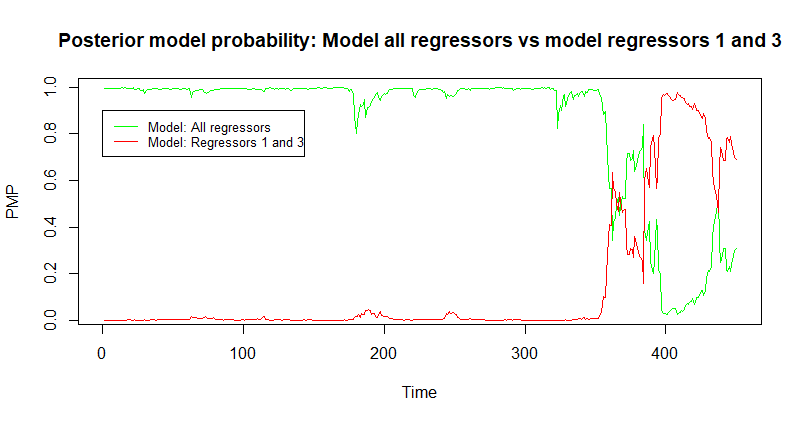
\includegraphics[width=340pt, height=200pt]{Chapters/chapter10/figures/figPMPdbma.png}
	\caption[List of figure caption goes here]{Posterior model probability: Dynamic Bayesian model averaging.}\label{figPMPdbma}
\end{figure}

Figures \ref{figPMPdbma1}, \ref{figPMPdbma2}, \ref{figPMPdbma3}, and \ref{figPMPdbma4} show a comparison between the Bayesian model averaging filtering recursions of the states (green lines) and their population values (red lines). We observe that the filtering recursions follow the general pattern of the population values. However, the values are not perfectly aligned. This discrepancy arises because the posterior model probabilities (PMPs) of the models that match the data-generating process are not equal to 1, which in turn affects the performance of the filtering recursions.  

\begin{figure}[!h]
	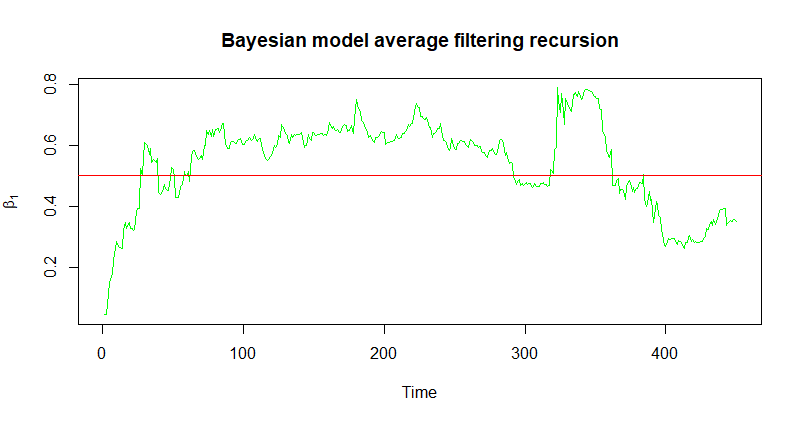
\includegraphics[width=340pt, height=200pt]{Chapters/chapter10/figures/figPMPdbma1.png}
	\caption[List of figure caption goes here]{State $\beta_{1}$: Population versus dynamic Bayesian model averaging of the filtering recursion.}\label{figPMPdbma1}
\end{figure}

\begin{figure}[!h]
	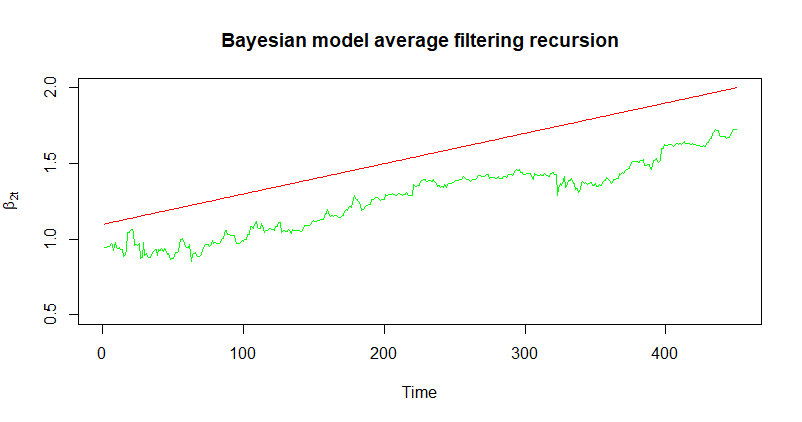
\includegraphics[width=340pt, height=200pt]{Chapters/chapter10/figures/figPMPdbma2.png}
	\caption[List of figure caption goes here]{State $\beta_{2t}$: Population versus dynamic Bayesian model averaging of the filtering recursion.}\label{figPMPdbma2}
\end{figure}

\begin{figure}[!h]
	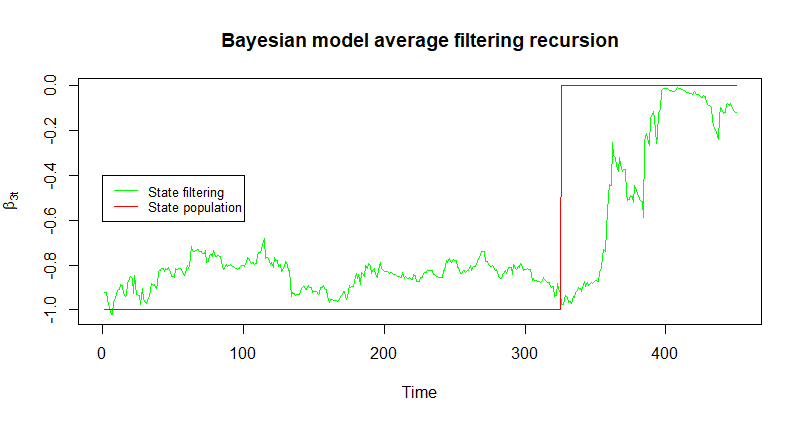
\includegraphics[width=340pt, height=200pt]{Chapters/chapter10/figures/figPMPdbma3.png}
	\caption[List of figure caption goes here]{State $\beta_{3t}$: Population versus dynamic Bayesian model averaging of the filtering recursion.}\label{figPMPdbma3}
\end{figure}

\begin{figure}[!h]
	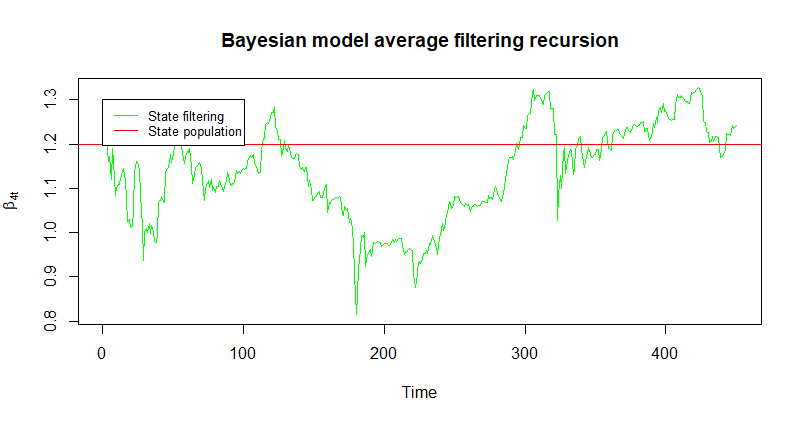
\includegraphics[width=340pt, height=200pt]{Chapters/chapter10/figures/figPMPdbma4.png}
	\caption[List of figure caption goes here]{State $\beta_{4}$: Population versus dynamic Bayesian model averaging of the filtering recursion.}\label{figPMPdbma4}
\end{figure}

Dynamic Bayesian model averaging was extended to logit models by \cite{mccormick2012dynamic}. We ask in Exercise 12 to perform a simulation of this model, and perform BMA using the function \textit{logistic.dma} from the \textit{dma} package.
     
\section{Generalized linear models}\label{sec10_3}

Generalized linear models (GLMs) were introduced by \cite{nelder1972generalized}, extending the concept of linear regression to a more general setting. These models are characterized by: i) a dependent variable $y_i$ whose probability distribution function belongs to the exponential family (see Section \ref{sec41}), ii) a linear predictor $\eta = \bm{x}^{\top}\bm{\beta}$, and iii) a link function such that $\mathbb{E}[y|\bm{x}] = g^{-1}(\bm{x}^{\top}\bm{\beta})$, which implies that $g(\mathbb{E}[y|\bm{x}]) = \bm{x}^{\top}\bm{\beta}$. GLMs can be extended to the overdispersed exponential family \cite{McCullagh1989}.

As we know from Section \ref{sec41}, the Poisson distribution belongs to the exponential family, such that $p(y|\lambda) = \frac{\exp(-\lambda)\exp(y\log(\lambda))}{y!}$, or in the canonical form $p(y|\eta) = \frac{\exp(\eta y - \exp(\eta))}{y!}$, where $\eta = \log(\lambda)$, which means that $\bm{x}^{\top}\bm{\beta} = \log(\lambda)$. Consequently, $\mathbb{E}[y|\bm{x}] = \nabla(\exp(\eta)) = \exp(\eta) = \lambda = \exp(\bm{x}^{\top}\bm{\beta})$. Therefore, the link function in the Poisson case is the \textit{log} function. In Exercise 6, we ask you to show that the link function in the Bernoulli case is the \textit{logit} function. Other examples include the identity function in the case of the Gaussian distribution and the negative inverse in the case of the gamma distribution.

We can use the GLM framework to perform Bayesian model averaging (BMA) using the BIC approximation, following \cite{Raftery1995}. Specifically, the BIC is given by $BIC = k_m \log(N) - 2 \log(p(\hat{\bm{\theta}}_m | \bm{y}))$, where $\hat{\bm{\theta}}_m$ is the maximum likelihood estimator. Thus, we simply need to calculate the likelihood function at the maximum likelihood estimator.\\

\textbf{Example: Simulation exercises}

Let's perform some simulation exercises to assess the performance of the BIC approximation using the Occam's window in GLMs. There are 27 regressors, where $x_{i1}$ and $x_{i2}$ are just the relevant regressors in all exercises, $i=1,2,\dots,1000$.
\begin{itemize}
	\item Logit: $x_k\sim N(0, 1)$, $k =1,\dots,27$, and $p(y_i=1|\bm{x}_i)=\exp(0.5+0.8x_{i1}-1.2x_{i2})/(1+\exp(0.5+0.8x_{i1}-1.2x_{i2}))$.
	
	\item Gamma: $x_k\sim N(0, 0.5^2)$, $k =1,\dots,27$, and $y_i\sim G(\alpha,\delta)$ where $\alpha=-(0.5+0.2x_{i1}0.1x_{i2})^{-1}$ and $\delta=1$.
	
	\item Poisson: $x_k\sim N(0, 1)$, $k =1,\dots,27$, and $\mathbb{E}[y_i|\bm{x}_i]=\lambda_i=\exp(0.5+1.1x_{i1}+0.7x_{i2})$.   
\end{itemize}

Our GUI uses the command \textit{bic.glm} from the \textit{BMA} package to perform BMA using the BIC approximation with the Occam's window in GLMs. The Algorithm \ref{alg:BMABIC} shows how to do this in our GUI, and the following code shows how to perform BMA in logit models using the simulation setting.

\begin{algorithm}[h!]
	\caption{Bayesian model averaging in generalized linear models using the Bayesian information criterion}\label{alg:BMABIC}
	\begin{algorithmic}[1]  		 			
		\State Select \textit{Bayesian Model Averaging} on the top panel
		\State Select the generalized linear model using the left radio button. Options: \textit{Binomial data (Logit)}, \textit{Real positive data (Gamma)} and \textit{Count data (Poisson)}
		\State Upload the dataset selecting first if there is header in the file, and the kind of separator in the \textit{csv} file of the dataset (comma, semicolon, or tab). Then, use the \textit{Browse} button under the \textbf{Choose File} legend
		\State Type the \textit{OR} number of the Occam's window in the box under \textbf{OR: Number between 5 and 50}, this is not necessary as by default there is 50
		\State Type the \textit{OL} number of the Occam's window in the box under \textbf{OL: Number between 0.0001 and 1}, this is not necessary as by default there is 0.0025
		\State Click the \textit{Go!} button
		\State Analyze results: After a few seconds or minutes, a table appears showing, for each regressor in the dataset, the PIP (posterior inclusion probability, \textbf{p!=0}), the BMA posterior mean (\textbf{EV}), the BMA standard deviation (\textbf{SD}), and the posterior mean for models with the highest PMP. At the bottom of the table, for the models with the largest PMP, the number of variables (\textbf{nVar}), the BIC, and the PMP (\textbf{post prob}) are displayed
		\State Download posterior results using the \textit{Download results using BIC}. There are two files, the first has the best models by row according to the PMP (last column) indicating with a 1 inclusion of the variable (0 indicates no inclusion), and the second file has the PIP, the BMA expected value and standard deviation for each variable in the dataset
	\end{algorithmic} 
\end{algorithm}

The results show that the PIPs of $x_{i1}$ and $x_{i2}$ are equal 1 in all three settings, the data generating process gets the highest PMP, and the BMA posterior means are close to the population values in each simulation setting. The other variables get PIPs close to 0, except a few exceptions, and the BMA posterior means are also close to 0. This suggests that the BIC approximation does a good job finding the data generating process in generalized linear models.
 
We can take advantage of the \textit{glm} function in \textbf{R} to perform BMA by programming an MC3 algorithm. The following code illustrates how to do this in the Poisson simulation. First, we simulate the data; second, we define a function to compute the log marginal likelihood approximation using the results from the \textit{glm} function. Then, we initialize the models to begin the MC3 algorithm. After that, we implement the MC3 algorithm, which involves small modifications of the code used for MC3 in Gaussian linear models.\footnote{Note that we have split the \textit{while} loop in the code into two pages.} We can calculate the posterior model probabilities (PMPs), posterior inclusion probabilities (PIPs), BMA means, and standard deviations as we did previously.

The simulation setting involves $2^{27}$ models, which corresponds to approximately 135 million models in the model space. We run our MC3 algorithm using the BIC approximation with 50,000 iterations. This takes considerably more time than the BIC approximation from the \textit{BMA} package, but it seems to perform well in identifying the data-generating process, as the PMP of this model equals 1. The posterior inclusion probabilities (PIPs) for $x_{i1}$ and $x_{i2}$ are also 1, and the posterior means are 1.1 and 0.7, respectively, which are equal to the population values. The t-ratios are far greater than 2. However, running 50,000 iterations results in mass concentration in one model, in this case, the data-generating process. If we run 25,000 MC3 iterations, the highest PMP is 0.8, but it is not associated with the data-generating process. Nonetheless, the PIP is equal to 1 for $x_{i1}$ and $x_{i2}$, and other regressors also have high PIPs. The BMA means for $x_{i1}$ and $x_{i2}$ are equal to the population values, and the BMA means for the other regressors are equal to 0. The t-ratios of the regressors in the population statistical model are much greater than 2, whereas the t-ratios of the other regressors are equal to 0. This exercise demonstrates that 25,000 iterations were not sufficient to uncover the data-generating process. However, it also emphasizes an important point: we need to analyze all the relevant results from the BMA analysis, not just the PMPs and/or PIPs.

In Exercise 10, we ask you to use this approach to perform a BMA algorithm in the logit regression, using the simulation setting for logit models from this section.

\begin{tcolorbox}[enhanced,width=4.67in,center upper,
	fontupper=\large\bfseries,drop shadow southwest,sharp corners]
	\textit{R code. Simulation exercise: BMA for generalized linear models}
	\begin{VF}
		\begin{lstlisting}[language=R]
			### Logit ###
			rm(list = ls()); set.seed(010101)
			n<-1000; B<-c(0.5,0.8,-1.2)
			X<-matrix(cbind(rep(1,n),rnorm(n,0,1),rnorm(n,0,1)),n,length(B))
			p <- exp(X%*%B)/(1+exp(X%*%B)); y <- rbinom(n, 1, p)
			nXgar<-25; Xgar<-matrix(rnorm(nXgar*n),n,nXgar)
			df<-as.data.frame(cbind(y,X[,-1],Xgar))
			colnames(df) <- c("y", "x1", "x2", "x3", "x4", "x5", "x6", "x7", "x8", "x9", "x10", "x11", "x12", "x13", "x14", "x15", "x16", "x17", "x18", "x19", "x20", "x21", "x22", "x23", "x24", "x25", "x26", "x27")
			BMAglmLogit <- BMA::bic.glm(y ~ x1+x2+x3+x4+x5+x6+x7+x8+x9+x10+x11+x12+x13+x14+x15+x16+x17+x18+x19+x20+x21+x22+x23+x24+x25+x26+x27, data = df, glm.family = binomial(link="logit"), strict = FALSE, OR = 50)
			summary(BMAglmLogit)
			### Gamma ###
			rm(list = ls()); set.seed(010101)
			n<-1000; B<- c(0.5, 0.2, 0.1)
			X<-matrix(cbind(rep(1,n),rnorm(n,0,0.5),rnorm(n,0,0.5)),n,length(B))
			y1 <- (X%*%B)^(-1)
			y <- rgamma(n,y1,scale=1)
			nXgar<-25; Xgar<-matrix(rnorm(nXgar*n),n,nXgar)
			df<-as.data.frame(cbind(y,X[,-1],Xgar))
			colnames(df) <- c("y", "x1", "x2", "x3", "x4", "x5", "x6", "x7", "x8", "x9", "x10", "x11", "x12", "x13", "x14", "x15", "x16", "x17", "x18", "x19", "x20", "x21", "x22", "x23", "x24", "x25", "x26", "x27")
			BMAglmGamma <- BMA::bic.glm(y ~ x1+x2+x3+x4+x5+x6+x7+x8+x9+x10+x11+x12+x13+x14+x15+x16+x17+x18+x19+x20+x21+x22+x23+x24+x25+x26+x27, data = df, glm.family = Gamma(link="inverse"), strict = FALSE, OR = 50)
			summary(BMAglmGamma)
			### Poisson ###
			rm(list = ls()); set.seed(010101)
			n<-1000; B<-c(2,1.1,0.7)
			X<-matrix(cbind(rep(1,n),rnorm(n,0,1),rnorm(n,0,1)),n,length(B))
			y1<-exp(X%*%B); y<-rpois(n,y1)
			nXgar<-25; Xgar<-matrix(rnorm(nXgar*n),n,nXgar)
			df<-as.data.frame(cbind(y,X[,-1],Xgar))
			colnames(df) <- c("y", "x1", "x2", "x3", "x4", "x5", "x6", "x7", "x8", "x9", "x10", "x11", "x12", "x13", "x14", "x15", "x16", "x17", "x18", "x19", "x20", "x21", "x22", "x23", "x24", "x25", "x26", "x27")
			BMAglmPoisson <- BMA::bic.glm(y ~ x1+x2+x3+x4+x5+x6+x7+x8+x9+x10+x11+x12+x13+x14+x15+x16+x17+x18+x19+x20+x21+x22+x23+x24+x25+x26+x27, data = df, glm.family = poisson(link="log"), strict = FALSE, OR = 50)
			summary(BMAglmPoisson)
		\end{lstlisting}
	\end{VF}
\end{tcolorbox} 


\begin{tcolorbox}[enhanced,width=4.67in,center upper,
	fontupper=\large\bfseries,drop shadow southwest,sharp corners]
	\textit{R code. Simulation exercise: BMA for generalized linear models using MC3 from scratch}
	\begin{VF}
		\begin{lstlisting}[language=R]
rm(list = ls()); set.seed(010101)
n<-1000; B<-c(2,1.1,0.7)
X<-matrix(cbind(rep(1,n),rnorm(n,0,1),rnorm(n,0,1)),n,length(B))
y1<-exp(X%*%B); y<-rpois(n,y1)
nXgar<-25; Xgar<-matrix(rnorm(nXgar*n),n,nXgar)
df<-as.data.frame(cbind(y,X[,-1],Xgar))
colnames(df) <- c("y", "x1", "x2", "x3", "x4", "x5", "x6", "x7", "x8", "x9", "x10", "x11", "x12", "x13", "x14", "x15", "x16", "x17", "x18", "x19", "x20", "x21", "x22", "x23", "x24", "x25", "x26", "x27")
Xnew <- apply(df[,-1], 2, scale)
BICfunt <- function(Model){
	indr <- Model == 1; kr <- sum(indr)
	if(kr > 0){
		Xr <- as.matrix(Xnew[ , indr])
		model <- glm(y ~ Xr, family = poisson(link = "log"))
		model_bic <- BIC(model)
		mllMod <- -model_bic/2
	}else{
		model <- glm(y ~ 1, family = poisson(link = "log"))
		model_bic <- BIC(model); mllMod <- -model_bic/2
	}
	return(mllMod)
}
M <- 500; K <- dim(df)[2] - 1
Models <- matrix(rbinom(K*M, 1, p = 0.5), ncol = K, nrow = M)
mllnew <- sapply(1:M, function(s){BICfunt(matrix(Models[s,], 1, K))})
oind <- order(mllnew, decreasing = TRUE)
mllnew <- mllnew[oind]; Models <- Models[oind, ]
# Hyperparameters MC3
iter <- 25000
pb <- winProgressBar(title = "progress bar", min = 0, max = iter, width = 300)
s <- 1
while(s <= iter){
	ActModel <- Models[M,]
	idK <- which(ActModel == 1)
	Kact <- length(idK)
	if(Kact < K & Kact > 1){
		CardMol <- K
		opt <- sample(1:3, 1)
		if(opt == 1){ # Same
			CandModel <- ActModel
		}else{
					if(opt == 2){ # Add
			All <- 1:K
			NewX <- sample(All[-idK], 1)
			CandModel <- ActModel
			CandModel[NewX] <- 1
		}else{ # Subtract
			LessX <- sample(idK, 1)
			CandModel <- ActModel
			CandModel[LessX] <- 0
		}
	}
\end{lstlisting}
	\end{VF}
\end{tcolorbox} 

\begin{tcolorbox}[enhanced,width=4.67in,center upper,
	fontupper=\large\bfseries,drop shadow southwest,sharp corners]
	\textit{R code. Simulation exercise: BMA for generalized linear models using MC3 from scratch}
	\begin{VF}
		\begin{lstlisting}[language=R]
	}else{
		CardMol <- K + 1
		if(Kact == K){
			opt <- sample(1:2, 1)
			if(opt == 1){ # Same
				CandModel <- ActModel
			}else{ # Subtract
				LessX <- sample(1:K, 1)
				CandModel <- ActModel
				CandModel[LessX] <- 0
			}
		}else{
			if(K == 1){
				opt <- sample(1:3, 1)
				if(opt == 1){ # Same
					CandModel <- ActModel
				}else{
					if(opt == 2){ # Add
						All <- 1:K
						NewX <- sample(All[-idK], 1)
						CandModel <- ActModel
						CandModel[NewX] <- 1
					}else{ # Subtract
						LessX <- sample(idK, 1)
						CandModel <- ActModel
						CandModel[LessX] <- 0
					}
				}
			}else{ # Add
				NewX <- sample(1:K, 1)
				CandModel <- ActModel
				CandModel[NewX] <- 1
			}
		}
	}
	LogMLact <- BICfunt(matrix(ActModel, 1, K))
	LogMLcand <- BICfunt(matrix(CandModel, 1, K))
	alpha <- min(1, exp(LogMLcand-LogMLact))
	u <- runif(1)
	if(u <= alpha){
		mllnew[M] <- LogMLcand
		Models[M, ] <- CandModel
		oind <- order(mllnew, decreasing = TRUE)
		mllnew <- mllnew[oind]
		Models <- Models[oind, ]
	}else{
		mllnew <- mllnew
		Models <- Models
	}
	s <- s + 1
	setWinProgressBar(pb, s, title=paste( round(s/iter*100, 0),"% done"))
}
close(pb)
\end{lstlisting}
	\end{VF}
\end{tcolorbox}   
 
\begin{tcolorbox}[enhanced,width=4.67in,center upper,
	fontupper=\large\bfseries,drop shadow southwest,sharp corners]
	\textit{R code. Simulation exercise: BMA for generalized linear models using MC3 from scratch}
	\begin{VF}
		\begin{lstlisting}[language=R]
ModelsUni <- unique(Models)
mllnewUni <- sapply(1:dim(ModelsUni)[1], function(s){BICfunt(matrix(ModelsUni[s,], 1, K))})
StMarLik <- exp(mllnewUni-mllnewUni[1])
PMP <- StMarLik/sum(StMarLik) # PMP based on unique selected models
plot(PMP)
ModelsUni[1,]
PIP <- NULL
for(k in 1:K){
	PIPk <- sum(PMP[which(ModelsUni[,k] == 1)])
	PIP <- c(PIP, PIPk)
}
plot(PIP)
Xnew <- df[,-1]
nModels <- dim(ModelsUni)[1]
Means <- matrix(0, nModels, K)
Vars <- matrix(0, nModels, K)
for(m in 1:nModels){
	idXs <- which(ModelsUni[m,] == 1)
	if(length(idXs) == 0){
		Regm <- glm(y ~ 1, family = poisson(link = "log"))
	}else{
		Xm <- as.matrix(Xnew[, idXs])
		Regm <- glm(y ~ Xm, family = poisson(link = "log"))
		SumRegm <- summary(Regm)
		Means[m, idXs] <- SumRegm[["coefficients"]][-1,1]
		Vars[m, idXs] <- SumRegm[["coefficients"]][-1,2]^2 
	}
}
BMAmeans <- colSums(Means*PMP)
BMAsd <- (colSums(PMP*Vars)  + colSums(PMP*(Means-matrix(rep(BMAmeans, each = nModels), nModels, K))^2))^0.5 
plot(BMAmeans)
plot(BMAsd)
plot(BMAmeans/BMAsd)
\end{lstlisting}
	\end{VF}
\end{tcolorbox}   
 
\section{Calculating the marginal likelihood}\label{sec10_4}

The BIC is an asymptotic approximation of the marginal likelihood, and consequently, it is used to obtain the Bayes factors. However, this method has limitations in applications with moderate and small sample sizes \cite{gelfand1994bayesian}. Therefore, other methods are available to calculate the Bayes factors when there is no analytical solution for the marginal likelihood.

Observe that calculating the Bayes factor with respect to a reference model ($\mathcal{M}_0$) helps to obtain the posterior model probabilities,

\begin{align*}
	\pi(\mathcal{M}_j |\bm{y})&=\frac{p(\bm{y} | \mathcal{M}_j)\pi(\mathcal{M}_j)}{\sum_{m=1}^{M}p(\bm{y} | \mathcal{M}_m)\pi(\mathcal{M}_m)}\\
	&=\frac{p(\bm{y} | \mathcal{M}_j)\pi(\mathcal{M}_j)/p(\bm{y} | \mathcal{M}_0)}{\sum_{m=1}^{M}p(\bm{y} | \mathcal{M}_m)\pi(\mathcal{M}_m)/p(\bm{y} | \mathcal{M}_0)}\\
	&=\frac{BF_{j0}\times\pi(\mathcal{M}_j)}{\sum_{m=1}^{M}BF_{l0}\times\pi(\mathcal{M}_l)}.
\end{align*}

Thus, $\pi(\mathcal{M}_j |\bm{y})=\frac{BF_{j0}}{\sum_{m=1}^{M}BF_{l0}}$ assuming equal prior model probabilities.

In addition, it has been established in many settings that the Bayes factor is consistent. That is, the probability of identifying the true data generating process converges to 1 as the sample size increases to infinity. Alternatively, it asymptotically identifies the model that minimizes the Kullback-Leibler divergence with respect to the data generating process when this process is not part of the models under consideration \cite{chib2016bayes, walker2004new, walker2004modern}.\footnote{\cite{Johnson2012} highlight the important distinction between pairwise consistency and model selection consistency. The latter requires the consistency of a sequence of pairwise nested comparisons.}

\subsection{Savage-Dickey density ratio}\label{sec10_4_1}

The Savage-Dickey density ratio is a way to calculate the Bayes factors when we compare nested models with particular priors \cite{dickey1971weighted,verdinelli1995computing}. In particular, given the parameter space $\bm{\theta}=(\bm{\omega}^{\top}, \bm{\psi}^{\top})^{\top}\in \bm{\Theta}=\bm{\Omega}\times \bm{\Psi}$, where we wish to test the null hypothesis $H_0:\bm{\omega}=\bm{\omega}_0$ (model $\mathcal{M}_1$) versus $H_1:\bm{\omega}\neq \bm{\omega}_0$ (model $\mathcal{M}_2$), if $\pi(\bm{\psi}|\bm{\omega}_0,\mathcal{M}_2)=\pi(\bm{\psi}|\mathcal{M}_1)$,\footnote{Note that a sufficient condition for this assumption is to assume the same prior for the parameters that are the same in each model. \cite{verdinelli1995computing} incorporate a correction factor when this assumption is not satisfied.} then the Bayes factor comparing $\mathcal{M}_1$ versus $\mathcal{M}_2$ is

\begin{equation}\label{eq:SD}
	BF_{12}=\frac{\pi(\bm{\omega}=\bm{\omega}_0|\bm{y},\mathcal{M}_2)}{\pi(\bm{\omega}=\bm{\omega}_0|\mathcal{M}_2)},
\end{equation}
where $\pi(\bm{\omega}=\bm{\omega}_0|\bm{y},\mathcal{M}_2)$ and $\pi(\bm{\omega}=\bm{\omega}_0|\mathcal{M}_2)$ are the posterior and prior densities of $\bm{\omega}$ under $\mathcal{M}_2$ evaluated at $\bm{\omega}_0$ (see \cite{verdinelli1995computing}). 

Equation \ref{eq:SD} is called the Savage-Dickey density ratio. A nice feature is that just requires estimation of model $\mathcal{M}_2$, and evaluation of the prior and posterior densities. This means no evaluation of the marginal likelihood \cite[Chap.~4]{koop2003bayesian}.\\

\subsection{Chib's methods}\label{sec10_4_2}

Another popular method to calculate the marginal likelihood is given by \cite{chib1995marginal} and \cite{chib2001marginal}. The former is an algorithm to calculate the marginal likelihood from the posterior draws of the Gibbs sampling algorithm, and the latter calculates the marginal likelihood from the posterior draws of the Metropolis-Hastings algorithm.

The point of departure in \cite{chib1995marginal} is the identity
\begin{align*}
	\pi(\bm{\theta}^*|\bm{y},\mathcal{M}_m)=\frac{p(\bm{y}|\bm{\theta}^*,\mathcal{M}_m)\times\pi(\bm{\theta}^*|\mathcal{M}_m)}{p(\bm{y}|\mathcal{M}_m)},
\end{align*} 
where $\bm{\theta}^*$ is a particular value of $\bm{\theta}$ of high probability, for instance, the mode. This implies that
\begin{align*}
	p(\bm{y}|\mathcal{M}_m)=\frac{p(\bm{y}|\bm{\theta}^*,\mathcal{M}_m)\times\pi(\bm{\theta}^*|\mathcal{M}_m)}{\pi(\bm{\theta}^*|\bm{y},\mathcal{M}_m)}.
\end{align*} 
We can easily calculate the numerator of this expression. However, the critical point in this expression is to calculate the denominator as we know $\pi(\bm{\theta}^*|\bm{y},\mathcal{M}_m)$ up to a normalizing constant. We can calculate this from the posterior draws. Assume that $\bm{\theta}=[\bm{\theta}^{\top}_1 \ \bm{\theta}^{\top}_2]^{\top}$, then $\pi(\bm{\theta}^*|\bm{y},\mathcal{M}_m)=\pi(\bm{\theta}^*_1|\bm{\theta}^*_2,\bm{y},\mathcal{M}_m)\times \pi(\bm{\theta}^*_2|\bm{y},\mathcal{M}_m)$. We have the first term because in the Gibbs sampling algorithm the posterior conditional distributions are available. The second is

\begin{align*}
	\pi(\bm{\theta}^*_2|\bm{y},\mathcal{M}_m)&=\int_{\bm{\Theta}_1}\pi(\bm{\theta}_1,\bm{\theta}^*_2|\bm{y},\mathcal{M}_m)d\bm{\theta}_1\\
	&=\int_{\bm{\Theta}_1}\pi(\bm{\theta}^*_2|\bm{\theta}_1,\bm{y},\mathcal{M}_m)\pi(\bm{\theta}_1|\bm{y},\mathcal{M}_m)d\bm{\theta}_1\\
	&\approx \frac{1}{S}\sum_{s=1}^S \pi(\bm{\theta}^*_2|\bm{\theta}^{(s)}_1,\bm{y},\mathcal{M}_m),
\end{align*} 

where $\bm{\theta}^{(s)}_1$ are the posterior draws of $\bm{\theta}_1$ from the Gibbs sampling algorithm. 

The generalization to more blocks can be seen in \cite{chib1995marginal} and \cite[Chap.~7]{greenberg2012introduction}. In addition, the extension to the Metropolis-Hastings algorithm can be seen in \cite{chib2001marginal}, and \cite[Chap.~7]{greenberg2012introduction}.

\subsection{Gelfand-Dey method}\label{sec10_4_3}
We can use the Gelfand-Dey method \cite{gelfand1994bayesian} when we want to calculate the Bayes factor to compare non-nested models, models where the Savage-Dickey density ratio is hard to calculate, or the Chib's methods are difficult to implement. The Gelfand-Dey method is very general, and can be used in virtually any model \cite[Chap.~5]{koop2003bayesian}.

Given a probability density function $q(\bm{\theta})$, whose support is in $\bm{\Theta}$, then
\begin{align*}
	\mathbb{E}\left[\frac{q(\bm{\theta})}{\pi(\bm{\theta}|\mathcal{M}_m)p(\bm{y}|\bm{\theta}_m,\mathcal{M}_m)}\biggr\rvert \bm{y},\mathcal{M}_m\right]&=\frac{1}{p(\bm{y}|\mathcal{M}_m)},
\end{align*} 

where the expected value is with respect to the posterior distribution given the model $\mathcal{M}_m$ (see Exercise 12).

The critical point is to select a good $q(\bm{\theta})$. \cite{geweke1999using} recommends to use $q(\bm{\theta})$ equal to a truncated multivariate normal density function with mean and variance equal to the posterior mean ($\hat{\bm{\theta}}$) and variance ($\hat{\bm{\Sigma}}$) of $\bm{\theta}$. The truncation region is $\hat{\bm{\Theta}}=\left\{\bm{\theta}:(\bm{\theta}-\hat{\bm{\theta}})^{\top}\hat{\bm{\Sigma}}^{-1}(\bm{\theta}-\hat{\bm{\theta}})\leq \chi_{1-\alpha}^2(K)\right\}$, where $\chi_{1-\alpha}^2(K)$ is the $(1-\alpha)$ percentile of the Chi-squared distribution with $K$ degrees of freedom, $K$ is the dimension of $\bm{\theta}$. We can pick small values of $\alpha$, for instance, $\alpha=0.01$.

Observe that 
\begin{align*}
	\mathbb{E}\left[\frac{q(\bm{\theta})}{\pi(\bm{\theta}|\mathcal{M}_m)p(\bm{y}|\bm{\theta}_m,\mathcal{M}_m)}\biggr\rvert \bm{y},\mathcal{M}_m\right]&\approx \frac{1}{S}\sum_{s=1}^S \left[\frac{q(\bm{\theta}^{(s)})}{\pi(\bm{\theta}^{(s)}|\mathcal{M}_m)p(\bm{y}|\bm{\theta}^{(s)}_m,\mathcal{M}_m)}\right],
\end{align*}
where $\bm{\theta}^{(s)}_m$ are draws from the posterior distribution.

Observe that we can calculate the marginal likelihoods of the models in Chapters \ref{chap6}, \ref{chap7}, \ref{chap8} and \ref{chap9} using the Chib's methods and the Gelfand-Dickey method.\\
    

\textbf{Example: Simulation exercise}

Let's check the performance of the Savage-Dickey density ratio, Chib's method and the Gelfand-Dey method to calculate the Bayes factor in a setting where we can obtain the analytical solution for the marginal likelihood. In particular, we will consider the Gaussian linear model with a conjugate prior (see Section \ref{sec43}).

Assume that the data generating process is given by  
\[
y_{i} = 0.7 + 0.3x_{i1} + 0.7x_{i2} - 0.2x_{i3} + 0.2x_{i4} + \mu_i,
\]
where \(x_{i1} \sim B(0.3)\), \(x_{ik} \sim N(0,1)\), for \(k = 2, \dots, 4\), and \(\mu_i \sim N(0, 1)\), for \(i = 1, 2, \dots, 500\). Let us set \(H_0: \beta_5 = 0\) (model \(\mathcal{M}_1\)) versus \(H_1: \beta_5 \neq 0\) (model \(\mathcal{M}_2\)).

We assume that \(\bm{\beta}_{m0} = \bm{0}_{m0}\), \(\bm{B}_{m0} = 0.5 \bm{I}_{m}\), \(\alpha_0 = \delta_0 = 4\). The dimensions of \(\bm{0}_{m0}\) and \(\bm{I}_m\) are 4 for model \(\mathcal{M}_1\) and 5 for model \(\mathcal{M}_2\). In addition, we assume equal prior probabilities for both models.

We know from Section \ref{sec43} that the marginal likelihood is
\begin{align*}
	p(\bf{y}|\mathcal{M}_m)&=\frac{\delta_{m0}^{\alpha_{m0}/2}}{\delta_{mn}^{\alpha_{mn}/2}}\frac{|{\bf{B}}_{mn}|^{1/2}}{|{\bf{B}}_{m0}|^{1/2}}\frac{\Gamma(\alpha_{mn}/2)}{\Gamma(\alpha_{m0}/2)},
\end{align*}
where  ${{\bm{B}}}_{mn} = ({\bm{B}}_{m0}^{-1} + {\bm{X}}_m^{\top}{\bm{X}}_m)^{-1}$, $\bm{\beta}_{mn} = {{\bf{B}}}_{mn}({\bm{B}}_{m0}^{-1}\bm{\beta}_{m0} + {\bm{X}}_m^{\top}{\bm{X}}_m\hat{\bm{\beta}}_m)$, $\alpha_{mn}=\alpha_{m0}+N$, and $\delta_{mn}=\delta_{m0}+({\bm{y}}-{\bm{X}}_m\hat{\bm{\beta}}_m)^{\top}({\bm{y}}-{\bm{X}}_m\hat{\bm{\beta}}_m)+(\hat{\bm{\beta}}_m-\bm{\beta}_{m0})^{\top}(({\bm{X}_m}^{\top}{\bm{X}_m})^{-1}+{\bm{B}}_{m0})^{-1}(\hat{\bm{\beta}}_m-\bm{\beta}_{m0})$, $m=1,2$ are the indices of the models.

The log marginal likelihoods for models $\mathcal{M}_1$ and $\mathcal{M}_2$ are -751.72 and -740.79, respectively. This implies a $2\times\log(BF_{21})=21.85$ which means positive evidence against model $\mathcal{M}_1$ (see Table \ref{tab:guide}).

We have different ways to calculate the Bayes factor using the Savage-Dickey density ratio in this example because we know that the marginal prior and marginal posterior distributions of $\beta_5$ have analytical solutions. In addition, we can use the posterior draws of $\sigma^2$ to evaluate the conditional prior and conditional posterior distributions at $\beta_5=0$. We show in the following code the latter approach, as it is more general than using analytical solutions, which are not always available.

We know that the conditional posterior distribution of $\beta_5$ is $N(\beta_{5n}, \sigma \bm{B}_{55n})$, where $\beta_{5n}$ is the 5th element of $\bm{\beta}_n$, and $\bm{B}_{55n}$ is the element 5,5 of $\bm{B}_n$. Then,
\begin{align*}
	\pi(\beta_5=0|\bm{y}, \mathcal{M}_2) &= \int_{\mathcal{R}^+} \pi(\beta_5=0|\bm{y}, \sigma^2) \pi(\sigma^2|\bm{y}) \, d\sigma^2 \\
	&\approx \frac{1}{S} \sum_{s=1}^S \pi(\beta_5=0|\bm{y}, \sigma^{2(s)}),
\end{align*}

where $\sigma^{2(s)}$ are draws from the posterior distribution of $\sigma^2$.

We can follow the same logic to obtain an approximation to $\pi(\beta_5=0|\mathcal{M}_2)$ by sampling draws from the prior distribution of $\sigma^2$.

We obtain $2 \times \log(BF_{21}) = 21.85$ using the Savage-Dickey density ratio, which is the same value as the analytic solution using the marginal likelihoods.
  

We calculate the log marginal likelihood using the Chib's method taking into account that 
\begin{align*}
	\log(p(\bm{y}|\mathcal{M}_m))&=\log(p(\bm{y}|\bm{\theta}^*,\mathcal{M}_m))+\log(\pi(\bm{\theta}^*|\mathcal{M}_m))-\log(\pi(\bm{\theta}^*|\bm{y},\mathcal{M}_m)),\\
\end{align*}
where $p(\bm{y}|\bm{\theta}^*,\mathcal{M}_m)$ is the value of a normal density with mean $\bm{X}_m\bm{\beta}_{m}^*$ and variance $\sigma^{2*}_m\bm{I}_N$ evaluated at $\bm{y}$. In addition, $\log(\pi(\bm{\theta}^*|\mathcal{M}_m))=\log(\pi(\bm{\beta}_m^*|\sigma^{2*}_m))+\log(\pi(\sigma^{2*}_m))$, where the first term is the density of a normal with mean $\bm{\beta}_{m0}$ and variance matrix $\sigma^{2*}\bm{B}_{m0}$ evaluated at $\bm{\beta}_m^*$, and the second term is the density of an inverse-gamma with parameters $\alpha_{m0}/2$ and $\delta_{m0}/2$ evaluated at $\sigma^{2*}_m$. Finally, the third term in the right hand of the previous expression is $\log(\pi(\bm{\theta}^*|\bm{y},\mathcal{M}_m))=\log(\pi(\bm{\beta}_m^*|\sigma^{2*}_m,\bm{y}))+\log(\pi(\sigma^{2*}_m|\bm{y}))$, where the first term is the density of a normal with mean $\bm{\beta}_{mn}$ and variance matrix $\sigma^{2*}_m\bm{B}_{mn}$ evaluated at $\bm{\beta}_m^*$, and the second term is the density of an inverse-gamma with parameters $\alpha_{mn}/2$ and $\delta_{mn}/2$ evaluated at $\sigma^{2*}_m$. We use the modes of the posterior draws of $\bm{\beta}_m$ and $\sigma^2_m$ as reference values. 

We get the same value, up to two decimals, for the log marginal likelihood of the restricted and unrestricted models using the Chib's method and the analytical expression. Thus, $2\times\log(BF_{21})=21.85$, that is, positive evidence against model $\mathcal{M}_1$ (see Table \ref{tab:guide}).

We calculate the log marginal likelihood using the Gelfand-Dey method taking into account that
\begin{align*}
	\log\left[\frac{q(\bm{\theta}^{(s)})}{\pi(\bm{\theta}^{(s)}|\mathcal{M}_m)p(\bm{y}|\bm{\theta}^{(s)}_m,\mathcal{M}_m)}\right]&=\log(q(\bm{\theta}^{(s)}))-\log(\pi(\bm{\theta}^{(s)}|\mathcal{M}_m))-\log(p(\bm{y}|\bm{\theta}^{(s)}_m,\mathcal{M}_m)),
\end{align*}
where $q(\bm{\theta}^{(s)})$ is the truncated multivariate normal density of Subsection \ref{sec10_4_3} evaluated at $\bm{\theta}^{(s)}=[\bm{\beta}^{(s)\top} \ \sigma^{2(s)}]^{\top}$, which is the $s$-th posterior draw of the Gibbs sampling algorithm, such that $\bm{\theta}^{(s)}$ satisfies the truncation restriction. $\log(\pi(\bm{\theta}^{(s)}|\mathcal{M}_m))=\log(\pi(\bm{\beta}_m^{(s)}|\sigma^{2(s)}_m))+\log(\pi(\sigma^{2(s)}_m))$, where the first term is the density of a normal with mean $\bm{\beta}_{m0}$ and variance matrix $\sigma^{2(s)}\bm{B}_{m0}$ evaluated at $\bm{\beta}_m^{(s)}$, and the second term is the density of an inverse-gamma with parameters $\alpha_{m0}/2$ and $\delta_{m0}/2$ evaluated at $\sigma^{2(s)}_m$. The third term $p(\bm{y}|\bm{\theta}^{(s)},\mathcal{M}_m)$ is the value of a normal density with mean $\bm{X}_m\bm{\beta}_{m}^{(s)}$ and variance $\sigma^{2(s)}_m\bm{I}_N$ evaluated at $\bm{y}$.

The log marginal likelihoods of the restricted and unrestricted models using the Gelfand-Dey method are -751.79 and -740.89, respectively. This implies $2\times \log(BF_{21})=21.81$, which is positive evidence in favor of the unrestricted model.

We see in this example that these methods give very good approximations to the true marginal likelihoods. However, the Savage-Dickey density ratio and Chib's method performed slightly better than the Gelfand-Dey method. In addition, the computational demand of the Gelfand-Dey method is by far the largest. This is because the Gelfand-Dey method requires many evaluations based on the posterior draws. However, we should keep in mind that the Gelfand-Dey method is more general.

The following code shows how to do all these calculations.

\begin{tcolorbox}[enhanced,width=4.67in,center upper,
	fontupper=\large\bfseries,drop shadow southwest,sharp corners]
	\textit{R code. Simulation exercise: Bayes factors}
	\begin{VF}
		\begin{lstlisting}[language=R]
rm(list = ls()); set.seed(010101)
N <- 500; K <- 5; K2 <- 3 
B <- c(0.7, 0.3, 0.7, -0.2, 0.2) 
X1 <- rbinom(N, 1, 0.3)
X2 <- matrix(rnorm(K2*N), N, K2)
X <- cbind(1, X1, X2)
Y <- X%*%B + rnorm(N, 0, sd = 1)
# Hyperparameters
d0 <- 4; a0 <- 4
b0 <- rep(0, K); cOpt <- 0.5
an <- N + a0; B0 <- cOpt*diag(K)
Bn <- solve(solve(B0)+t(X)%*%X); bhat <- solve(t(X)%*%X)%*%t(X)%*%Y
bn <- Bn%*%(solve(B0)%*%b0+t(X)%*%X%*%bhat)
dn <- as.numeric(d0 + t(Y-X%*%bhat)%*%(Y-X%*%bhat)+t(bhat - b0)%*%solve(solve(t(X)%*%X)+B0)%*%(bhat - b0))
Hn <- as.matrix(Matrix::forceSymmetric(dn*Bn/an))
S <- 10000
LogMarLikLM <- function(X, c0){
	K <- dim(X)[2]
	N <- dim(X)[1]	
	# Hyperparameters
	B0 <- c0*diag(K)
	b0 <- rep(0, K)
	# Posterior parameters
	bhat <- solve(t(X)%*%X)%*%t(X)%*%Y
	# Force this matrix to be symmetric
	Bn <- as.matrix(Matrix::forceSymmetric(solve(solve(B0) + t(X)%*%X))) 
	bn <- Bn%*%(solve(B0)%*%b0 + t(X)%*%X%*%bhat)
	dn <- as.numeric(d0 + t(Y)%*%Y+t(b0)%*%solve(B0)%*%b0-t(bn)%*%solve(Bn)%*%bn)
	an <- a0 + N
	# Log marginal likelihood
	logpy <- (N/2)*log(1/pi)+(a0/2)*log(d0)-(an/2)*log(dn) + 0.5*log(det(Bn)/det(B0)) + lgamma(an/2)-lgamma(a0/2)
	return(-logpy)
}
LogMarM2 <- -LogMarLikLM(X = X, c0 = cOpt)
LogMarM1 <- -LogMarLikLM(X = X[,1:4], c0 = cOpt)
BF12 <- exp(LogMarM1-LogMarM2) 
BF12; 1/BF12
2*log(1/BF12)
# Savage-Dickey density ratio
# Posterior evaluation
Brest <- 0
sig2P <- invgamma::rinvgamma(S, shape = an/2, rate = dn/2)
PostRestCom <- mean(sapply(sig2P, function(x){dnorm(Brest, mean = bn[5], sd = (x*Bn[5,5])^0.5, log = FALSE)})) 
# Prior evaluation
sig2 <- invgamma::rinvgamma(S, shape = a0/2, rate = d0/2)
PriorRestCom <- mean(sapply(sig2, function(x){dnorm(Brest, mean = 0, sd = (x*cOpt)^0.5, log = FALSE)})) 
# Bayes factor
BF12SD <- PostRestCom/PriorRestCom
2*log(1/BF12SD)
\end{lstlisting}
	\end{VF}
\end{tcolorbox}            


\begin{tcolorbox}[enhanced,width=4.67in,center upper,
	fontupper=\large\bfseries,drop shadow southwest,sharp corners]
	\textit{R code. Simulation exercise: Bayes factors}
	\begin{VF}
		\begin{lstlisting}[language=R]
# Chib's method
sig2Post <- MCMCpack::rinvgamma(S,an/2,dn/2)
BetasGibbs <- sapply(1:S, function(s){MASS::mvrnorm(n = 1, mu = bn, Sigma = sig2Post[s]*Bn)})
# Mode function for continuous data
mode_continuous <- function(x){
	density_est <- density(x)       
	mode_value <- density_est$x[which.max(density_est$y)]  
	return(mode_value)
}
# Unrestricted model
BetasMode <- apply(BetasGibbs, 1, mode_continuous)
Sigma2Mode <- mode_continuous(sig2Post)
VarModel <- Sigma2Mode*diag(N)
MeanModel <- X%*%BetasMode
LogLik <- mvtnorm::dmvnorm(c(Y), mean = MeanModel, sigma = VarModel, log = TRUE, checkSymmetry = TRUE)
LogPrior <- mvtnorm::dmvnorm(BetasMode, mean = rep(0, K), sigma = Sigma2Mode*cOpt*diag(K), log = TRUE, checkSymmetry = TRUE)+log(MCMCpack::dinvgamma(Sigma2Mode, a0/2, d0/2))
LogPost1 <- mvtnorm::dmvnorm(BetasMode, mean = bn, sigma = Sigma2Mode*Bn, log = TRUE, checkSymmetry = TRUE)
LogPost2 <- log(MCMCpack::dinvgamma(Sigma2Mode, an/2, dn/2))
LogMarLikChib <- LogLik + LogPrior -(LogPost1 + LogPost2)
# Restricted model
anRest <- N + a0; XRest <- X[,-5]
KRest <- dim(XRest)[2]; B0Rest <- cOpt*diag(KRest) 
BnRest <- solve(solve(B0Rest)+t(XRest)%*%XRest)
bhatRest <- solve(t(XRest)%*%XRest)%*%t(XRest)%*%Y
b0Rest <- rep(0, KRest)
bnRest <- BnRest%*%(solve(B0Rest)%*%b0Rest+t(XRest)%*%XRest%*%bhatRest)
dnRest <- as.numeric(d0 + t(Y-XRest%*%bhatRest)%*%(Y-XRest%*%bhatRest)+t(bhatRest - b0Rest)%*%solve(solve(t(XRest)%*%XRest)+B0Rest)%*%(bhatRest - b0Rest))
sig2PostRest <- MCMCpack::rinvgamma(S,anRest/2,dnRest/2)
BetasGibbsRest <- sapply(1:S, function(s){MASS::mvrnorm(n = 1, mu = bnRest, Sigma = sig2PostRest[s]*BnRest)})
BetasModeRest <- apply(BetasGibbsRest, 1, mode_continuous)
Sigma2ModeRest <- mode_continuous(sig2PostRest)
VarModelRest <- Sigma2ModeRest*diag(N)
MeanModelRest <- XRest%*%BetasModeRest
LogLikRest <- mvtnorm::dmvnorm(c(Y), mean = MeanModelRest, sigma = VarModelRest, log = TRUE, checkSymmetry = TRUE)
LogPriorRest <- mvtnorm::dmvnorm(BetasModeRest, mean = rep(0, KRest), sigma = Sigma2ModeRest*cOpt*diag(KRest), log = TRUE, checkSymmetry = TRUE)+log(MCMCpack::dinvgamma(Sigma2ModeRest, a0/2, d0/2))
LogPost1Rest <- mvtnorm::dmvnorm(BetasModeRest, mean = bnRest, sigma = Sigma2ModeRest*BnRest, log = TRUE, checkSymmetry = TRUE)
LogPost2Rest <- log(MCMCpack::dinvgamma(Sigma2ModeRest, anRest/2, dnRest/2))
LogMarLikChibRest <- LogLikRest + LogPriorRest -(LogPost1Rest + LogPost2Rest)
BFChibs <- exp(LogMarLikChibRest-LogMarLikChib)
BFChibs; 1/BFChibs; 2*log(1/BFChibs)
\end{lstlisting}
\end{VF}
\end{tcolorbox}

\begin{tcolorbox}[enhanced,width=4.67in,center upper,
	fontupper=\large\bfseries,drop shadow southwest,sharp corners]
	\textit{R code. Simulation exercise: Bayes factors}
	\begin{VF}
		\begin{lstlisting}[language=R]
# Gelfand-Dey method
GDmarglik <- function(ids, X, Betas, MeanThetas, VarThetas, sig2Post){
	K <- dim(X)[2]; Thetas <- c(Betas[ids,], sig2Post[ids])
	Lognom <- (1/(1-alpha))*mvtnorm::dmvnorm(Thetas, mean = MeanThetas, sigma = VarThetas, log = TRUE, checkSymmetry = TRUE)
	Logden1 <- mvtnorm::dmvnorm(Betas[ids,], mean = rep(0, K), sigma = sig2Post[ids]*cOpt*diag(K), log = TRUE, checkSymmetry = TRUE) + log(MCMCpack::dinvgamma(sig2Post[ids], a0/2, d0/2))
	VarModel <- sig2Post[ids]*diag(N)
	MeanModel <- X%*%Betas[ids,]
	Logden2 <- mvtnorm::dmvnorm(c(Y), mean = MeanModel, sigma = VarModel, log = TRUE, checkSymmetry = TRUE)
	LogGDid <- Lognom - Logden1 - Logden2
	return(LogGDid)
}
sig2Post <- MCMCpack::rinvgamma(S,an/2,dn/2)
Betas <- LaplacesDemon::rmvt(S, bn, Hn, an)
Thetas <- cbind(Betas, sig2Post)
MeanThetas <- colMeans(Thetas); VarThetas <- var(Thetas)
iVarThetas <- solve(VarThetas)
ChiSQ <- sapply(1:S, function(s){(Thetas[s,]-MeanThetas)%*%iVarThetas%*%(Thetas[s,]-MeanThetas)})
alpha <- 0.01; criticalval <- qchisq(1-alpha, K + 1)
idGoodThetas <- which(ChiSQ <= criticalval)
pb <- winProgressBar(title = "progress bar", min = 0, max = S, width = 300)
InvMargLik2 <- NULL
for(s in idGoodThetas){
	LogInvs <- GDmarglik(ids = s, X = X, Betas = Betas, MeanThetas = MeanThetas, VarThetas = VarThetas, sig2Post = sig2Post)
	InvMargLik2 <- c(InvMargLik2, LogInvs)
	setWinProgressBar(pb, s, title=paste( round(s/S*100, 0),"% done"))
}
close(pb); mean(InvMargLik2)
# Restricted model
anRest <- N + a0; XRest <- X[,-5]
KRest <- dim(XRest)[2]; B0Rest <- cOpt*diag(KRest) 
BnRest <- solve(solve(B0Rest)+t(XRest)%*%XRest)
bhatRest <- solve(t(XRest)%*%XRest)%*%t(XRest)%*%Y
b0Rest <- rep(0, KRest)
bnRest <- BnRest%*%(solve(B0Rest)%*%b0Rest+t(XRest)%*%XRest%*%bhatRest)
dnRest <- as.numeric(d0 + t(Y-XRest%*%bhatRest)%*%(Y-XRest%*%bhatRest)+t(bhatRest - b0Rest)%*%solve(solve(t(XRest)%*%XRest)+B0Rest)%*%(bhatRest - b0Rest))
HnRest <- as.matrix(Matrix::forceSymmetric(dnRest*BnRest/anRest))
sig2PostRest <- MCMCpack::rinvgamma(S,anRest/2,dnRest/2)
BetasRest <- LaplacesDemon::rmvt(S, bnRest, HnRest, anRest)
ThetasRest <- cbind(BetasRest, sig2PostRest)
MeanThetasRest <- colMeans(ThetasRest)
VarThetasRest <- var(ThetasRest)
iVarThetasRest <- solve(VarThetasRest)
\end{lstlisting}
	\end{VF}
\end{tcolorbox}  

\begin{tcolorbox}[enhanced,width=4.67in,center upper,
	fontupper=\large\bfseries,drop shadow southwest,sharp corners]
	\textit{R code. Simulation exercise: Bayes factors}
	\begin{VF}
		\begin{lstlisting}[language=R]
ChiSQRest <- sapply(1:S, function(s){(ThetasRest[s,]-MeanThetasRest)%*%iVarThetasRest%*%(ThetasRest[s,]-MeanThetasRest)})
idGoodThetasRest <- which(ChiSQRest <= criticalval)
pb <- winProgressBar(title = "progress bar", min = 0, max = S, width = 300)
InvMargLik1 <- NULL
for(s in idGoodThetasRest){
	LogInvs <- GDmarglik(ids = s, X = XRest, Betas = BetasRest, MeanThetas = MeanThetasRest, VarThetas = VarThetasRest, sig2Post = sig2PostRest)
	InvMargLik1 <- c(InvMargLik1, LogInvs)
	setWinProgressBar(pb, s, title=paste( round(s/S*100, 0),"% done"))
}
close(pb); summary(coda::mcmc(InvMargLik1))
mean(InvMargLik1)
BFFD <- exp(mean(InvMargLik2)-mean(InvMargLik1))
BFFD; mean(1/BFFD); 2*log(1/BFFD)
\end{lstlisting}
	\end{VF}
\end{tcolorbox}  

\begin{comment}
The Bayes factor using the Savage-Dickey density ratio is

\begin{align*}
	BF_{12}&=\frac{\pi(\bm{\beta}_{5}=\bm{0}_2|\bm{y},\mathcal{M}_2)}{\pi(\bm{\beta}_{5}=\bm{0}_2|\mathcal{M}_2)},
\end{align*}
where $\pi(\bm{\beta}_{5}=\bm{0}_2|\bm{y},\mathcal{M}_2)$ is the density of a  student's t-distribution with mean equal to the last element of $\bm{\beta}_{2n}$, scale parameter $\bm{H}_{2n,5,5}$, that is, the element 5:5 of the matrix $\bm{H}_{2n}$, where $\bm{H}_{2n}=\delta_{2n}\bm{B}_{2n}/\alpha_{2n}$, and degrees of freedom $\alpha_{2n}$.

Given that the prior distribution of $\bm{\beta}|\sigma^2$ is $N(\bm{\beta}_0,\sigma^2\bm{B}_0)$, this implies that $\bm{\beta}_{5}|\sigma^2\sim N(\bm{\beta}_{0,5},\sigma^2\bm{B}_{0,5,5})$. Then,
\begin{align*}
	\pi(\bm{\beta}_{5}|\mathcal{M}_2)&=\int_{0}^{\infty}(2\pi\sigma^2)^{-1/2}|\bm{B}_0|^{-1/2}\exp\left\{-\frac{1}{2\sigma^2}(\bm{\beta}_{4:5}-\bm{\beta}_{0,4:5})^{\top}\bm{B}_{0,4:5}^{-1}(\bm{\beta}_{4:5}-\bm{\beta}_{0,4:5})\right\}\\
	&\times \frac{(\delta_0/2)^{\alpha_0/2}}{\Gamma(\alpha_0/2)}\left(\frac{1}{\sigma^2}\right)^{\alpha_0/2+1}\exp \left\{-\frac{\delta_0}{2\sigma^2} \right\}d\sigma^2
\end{align*}
\end{comment}

\begin{comment}
	Given the prior specification of Section \ref{sec10_2}, the Bayes factor is
	\begin{align*}
		BF_{12}&=\frac{\left(\frac{g_1}{1+g_1}\right)^{k_1/2} \left[(\bm{y}-\bar{y}\bm{i}_N)^{\top}(\bm{y}-\bar{y}\bm{i}_N)-\frac{1}{1+g_1}(\bm{y}^{\top}\bm{P}_{X_1}\bm{y})\right]^{-(N-1)/2}}{\left(\frac{g_2}{1+g_2}\right)^{k_2/2} \left[(\bm{y}-\bar{y}\bm{i}_N)^{\top}(\bm{y}-\bar{y}\bm{i}_N)-\frac{1}{1+g_2}(\bm{y}^{\top}\bm{P}_{X_2}\bm{y})\right]^{-(N-1)/2}},
	\end{align*}
	where $\bm{P}_{X_m}=\bm{X}_m(\bm{X}_m^{\top}\bm{X}_m)^{-1}\bm{X}_m$ is the projection matrix on the space generated by the columns of $\bm{X}_m$, $m=1,2$. In particular, $k_1=2$, $k_2=4$, $\bm{X}_1$ does not take into account $x_{i3}$ neither $x_{i4}$, whereas $\bm{X}_2$ takes into account all the regressors.
	
	The Bayes factor of the restricted model versus the unrestricted model is equal to 0.0129. This is strong evidence against model $\mathcal{M}_1$ according to the Kass and Raftery guidelines (see Table \ref{tab:guide}). 
	
	Let's calculate the Bayes factor using the Savage-Dickey density ration. We have in this setting
	\begin{align*}
		\pi(\bm{\beta}=\bm{0}_{0m}|\mathcal{M}_2)&=(2\pi\sigma^2)^{-2/7}|g_m\bm{X}_m^{\top}\bm{X}_m|^{-1/2}\\
		&\times\exp\left\{-\frac{1}{2\sigma^2}(\bm{0}_{0m}-\bm{\beta}_{0})^{\top}(g_m\bm{X}_m^{\top}\bm{X}_m)^{-1}(\bm{0}_{0m}-\bm{\beta}_{0})\right\}
	\end{align*}  
	
	We know that the marginal likelihood function of the linear Gaussian model with independent priors does not have an analytical solution. Then, let's perform a simulation exercise assuming that there are five fixed regressors, for instance, factors in treatment effects, and other five additional regressors that we are not sure about their relevance in the model. We can use BMA in this setting to check robustness of the treatment factors regarding the model specification associated with the other five regressors.
	
	Let's assume that the data generating process is $y_{it}=0.8+0.3x_{i3}+0.7x_{i7}-0.5x_{10i}+\mu_i$, where $\bm{x}_{i}\sim B(5, \bm{p})$, $\bm{p}=[0.1 \ 0.3 \ 0.3 \ 0.2 \ 0.1]^{\top}$, $x_{ik}\sim N(0,1)$, $k=6,\dots,10$, and $y_i=0.7+0.3x_{i3}+0.7x_{i7}-0.5x_{i10}+\mu_i$, $\mu_i\sim N(0,1)$.
	
	
	
	
	where all parameter are indexed to model $\mathcal{M}_m$, $\bm{P}_{X_m}=\bm{X}_m(\bm{X}_m^{\top}\bm{X}_m)^{-1}\bm{X}_m$ is the projection matrix on the space generated by the columns of $\bm{X}_m$, and $\bar{y}$ is the sample mean of $\bm{y}$. 
	
	In the Gaussian linear model with independent priors (see Section \ref{sec62}), we have ${\bf{y}}={\bf{X}}\bm{\bm{\beta}}+\bm{\mu}$ such that $\bm{\mu}\sim N(\bf{0},\sigma^2\bf{I}_N)$, $\bm{\beta} \sim N(\bm{\beta}_0, {\bf{B}}_0)$ and $\sigma^2 \sim IG(\alpha_0/2, \delta_0/2)$. Then, $\bm{\beta}|\sigma^2, {\bf{y}}, {\bf{X}} \sim N(\bm{\beta}_n, \sigma^2{\bf{B}}_n)$ and $\sigma^2|\bm{\beta}, {\bf{y}}, {\bf{X}} \sim IG(\alpha_n/2, \delta_n/2)$, where  ${\bf{B}}_n = ({\bf{B}}_0^{-1} + \sigma^{-2} {\bf{X}}^{\top}{\bf{X}})^{-1}$, $\bm{\beta}_n= {\bf{B}}_n({\bf{B}}_0^{-1}\bm{\beta}_0 + \sigma^{-2} {\bf{X}}^{\top}{\bf{y}})$, $\alpha_n = \alpha_0 + N$ and $\delta_n = \delta_0 + ({\bf{y}}-{\bf{X}}\bm{\beta})^{\top}({\bf{y}}-{\bf{X}}\bm{\beta})$.
	
	We can use as reference the model with all the regressors. Then,
	\begin{align*}
		\pi(\bm{\beta}=\bm{0}_{0k}|\mathcal{M}_2)=(2\pi)^{-2/10}|\bm{B}_{0}|^{-1/2}\exp\left\{-\frac{1}{2}(\bm{0}_{0k}-\bm{\beta}_{0})^{\top}\bm{B}_{0}^{-1}(\bm{0}_{0k}-\bm{\beta}_{0})\right\}
	\end{align*}  
	
	\begin{align*}
		\pi(\bm{\beta}=\bm{0}_{0m}|\mathcal{M}_2)&=(2\pi\sigma^2)^{-2/7}|g_m\bm{X}_m^{\top}\bm{X}_m|^{-1/2}\\
		&\times\exp\left\{-\frac{1}{2\sigma^2}(\bm{0}_{0m}-\bm{\beta}_{0})^{\top}(g\bm{X}_m^{\top}\bm{X}_m)^{-1}(\bm{0}_{0m}-\bm{\beta}_{0})\right\}
	\end{align*}  
\end{comment}
    

\section{Summary}\label{sec10_5}
In this chapter, we introduced Bayesian model averaging (BMA) in generalized linear models. For linear Gaussian models, we perform BMA using three approaches: the Bayesian Information Criterion (BIC) approximation with Occam's window, the Markov Chain Monte Carlo Model Composition (MC3) algorithm, and conditional Bayes factors, which account for endogeneity. For other generalized linear models, such as logit, gamma, and Poisson, we demonstrate how to use the BIC approximation to perform BMA. Additionally, we show how to perform dynamic Bayesian model averaging in state-space models, where forgetting parameters are used to facilitate computation. Finally, we present alternative methods for calculating the marginal likelihood: the Savage-Dickey density ratio, Chib's method, and the Gelfand-Dey method. These methods are particularly useful when the BIC approximation does not perform well due to small or moderate sample sizes.

\section{Exercises}\label{sec10_6}

\begin{enumerate}
	\item The Gaussian linear model specifies $\bf{y}=\alpha\bm{i}_N+\bm{X}_m\bm{\beta}_m+\bm{\mu}_m$ such that $\bm{\mu}_m\sim{N}(\bm{0},\sigma^2\bm{I}_n)$, and $\bm{X}_m$ does not have the column of ones. Assuming that $\pi(\sigma^2)\propto 1/{\sigma^2}$, $\pi(\alpha)\propto 1$, and $\bm{\beta}_m|\sigma^2 \sim {N}(\bm{0}_{k_m}, \sigma^2 (g_m\bm{X}_m^{\top}\bm{X}_m)^{-1})$.
	\begin{itemize}
		\item Show that the posterior conditional distribution of $\bm{\beta}_m$ is $N(\bm{\beta}_{mn},\sigma^2\bm{B}_{mn})$, where $\bm{\beta}_{mn}=\bm{B}_{mn}\bm{X}_m^{\top}\bm{y}$ and $\bm{B}_{mn}=((1+g_m)\bm{X}_m^{\top}\bm{X}_m)^{-1}$.
		\item Show that the marginal likelihood associated with model $\mathcal{M}_m$ is proportional to
		\begin{align*}
			p(\bm{y}|\mathcal{M}_m)&\propto \left(\frac{g_m}{1+g_m}\right)^{k_m/2} \left[(\bm{y}-\bar{y}\bm{i}_N)^{\top}(\bm{y}-\bar{y}\bm{i}_N)-\frac{1}{1+g_m}(\bm{y}^{\top}\bm{P}_{X_m}\bm{y})\right]^{-(N-1)/2},
		\end{align*}
		where all parameter are indexed to model $\mathcal{M}_m$, $\bm{P}_{X_m}=\bm{X}_m(\bm{X}_m^{\top}\bm{X}_m)^{-1}\bm{X}_m$ is the projection matrix on the space generated by the columns of $\bm{X}_m$, and $\bar{y}$ is the sample mean of $\bm{y}$.
		
		Hint: Take into account that $\bm{i}_N^{\top}\bm{X}_m=\bm{0}_{k_m}$ due to all columns being centered with respect to their means.
	\end{itemize}

\item \textbf{Determinants of export diversification I}

\cite{Jetter2015} use BMA to study the determinants of export diversification. Use the dataset \textit{10ExportDiversificationHHI.csv} to perform BMA using the BIC approximation and MC3 to check if these two approaches agree. 

\item \textbf{Simulation exercise of the Markov chain Monte Carlo model composition continues}

Program an algorithm to perform MC3 where the final $S$ models are unique. Use the simulation setting of Section \ref{sec10_2} increasing the number of regressors to 40, this implies approximately 1.1e+12 models.

\item \textbf{Simulation exercise of IV BMA continues}

Use the simulation setting with endogeneity in Section \ref{sec10_2} to perform BMA based on the BIC approximation and MC3.

\item \textbf{Determinants of export diversification II}

Use the datasets \textit{11ExportDiversificationHHI.csv} and \textit{12ExportDiversificationHHIInstr.csv} to perform IV BMA assuming that the log of per capita gross domestic product is endogenous (\textit{avglgdpcap}). See \cite{Jetter2015} for details.

\item Show that the link function in the case of the Bernoulli distribution is $\log\left(\frac{\theta}{1-\theta}\right)$.

\item \cite{ramirez2020dynamic, ramirez2021specification} perform variable selection using the file \textit{13InternetMed.csv}. In this dataset, the dependent variable is an indicator of Internet adoption (\textit{internet}) for 5,000 households in Medell\'in (Colombia) during the period 2006--2014. This dataset contains information about 18 potential determinants, which implies 262,144 ($2^{18}$) potential models, considering only variable uncertainty (see these papers for details about the dataset). Perform BMA using the logit link function with this dataset.  

\item \cite{Serna2018} use the file \textit{14ValueFootballPlayers.csv} to analyze the market value of soccer players in the most important leagues in Europe. In particular, there are 26 potential determinants of the market value (dependent variable) of a stratified sample of 335 soccer players from the five most important leagues in Europe (see \cite{Serna2018} for details). Use this dataset to perform BMA using the gamma distribution, setting the default values for Occam's window.  

\item Use the dataset \textit{15Fertile2.csv} from \cite[p.~547]{Wooldridge2012} to perform BMA using the Poisson model with the log link. This dataset contains information about 1,781 women from Botswana in 1988 (for details, see \textbf{https://rdrr.io/cran/wooldridge/man/fertil2.html}), with the caveat that we deleted some variables and omitted observations with NA values. The dependent variable is the number of children ever born (\texttt{ceb}), which is a count variable, as a function of 19 potential determinants.

\item Perform BMA in the logit model using MC3 and the BIC approximation using the simulation setting of Section \ref{sec10_3}.

\item Use the dataset \textit{19ExchangeRateCOPUSD.csv} to estimate four different \textit{state-space models} to explain the annual variation of the COP to USD exchange rate: 
\begin{itemize}
	\item Interest rate parity
	
	$\Delta e_t = \beta_{1t}^{IRP} + \beta_{2t}^{IRP} (i_{t-1}^{Col}-i_{t-1}^{USA})+\mu_{t}^{IRP}$ 
	\item Purchasing power parity
	
	$\Delta e_t = \beta_{1t}^{PPP} + \beta_{2t}^{PPP} (\pi_{t-1}^{Col}-\pi_{t-1}^{USA})+\mu_{t}^{PPP}$
	\item Taylor rule
	
	$\Delta e_t = \beta_{1t}^{Taylor} + \beta_{2t}^{Taylor} (\pi_{t-1}^{Col}-\pi_{t-1}^{USA})+\beta_{2t}^{Taylor} (g_{t-1}^{Col}-g_{t-1}^{USA})+\mu_{t}^{IRP}$
	\item Money supply
	
	$\Delta e_t = \beta_{1t}^{Money} + \beta_{2t}^{Money} (g_{t-1}^{Col}-g_{t-1}^{USA})+\beta_{2t}^{Money} (m_{t-1}^{Col}-m_{t-1}^{USA})+\mu_{t}^{Money}$   
\end{itemize}
where \textit{varTRM} ($\Delta e_t$) represents the annual variation rate of the exchange rate from COP to USD, \textit{TES\_COL10} ($i_{t}^{Col}$) and \textit{TES\_USA10} ($i_{t}^{USA}$) denote the annual return rates of Colombian and U.S. public debts over 10 years, \textit{inflation\_COL} ($\pi_{t}^{Col}$) and \textit{inflation\_USA} ($\pi_{t}^{USA}$) are the annual inflation rates for Colombia and the U.S., \textit{varISE\_COL} ($g_{t}^{Col}$) and \textit{varISE\_USA} ($g_{t}^{USA}$) represent the annual variations of economic activity indices, and \textit{varCOL\_M3} ($m_{t}^{Col}$) and \textit{varUSA\_M3} ($m_{t}^{USA}$) are the annual variations of the money supply. The dataset includes monthly variations from January 2006 to November 2023.

Perform Bayesian model averaging using these four models to explain the annual variation of the exchange rate, calculate the posterior model probabilities, and plot the posterior mean and credible interval of $\beta_{2t}^{Money}$.   

\item Perform a simulation of the dynamic logistic model, where there are 7 ($2^3 - 1$, excluding the model without regressors) competing models originating from 3 regressors: $x_{tk} \sim N(0.5, 0.8^2)$, $k = 2, 3, 4$, and $\beta_1 = 0.5$, $\beta_{2t}$ is a sequence from 1 to 2 in steps given by $1/T$, and $\beta_{3t} = \begin{Bmatrix}
	-1, & 1 < t \leq 0.5T \\
	0, & 0.5T < t \leq T
\end{Bmatrix}$, with $\beta_4 = 1.2$. Then, $\bm{x}_t^{\top} \bm{\beta}_t = \beta_1 + \beta_{2t} x_{2t} + \beta_{3t} x_{3t} + \beta_4 x_{4t}$, where 
\[
P[Y_t = 1 | \bm{x}_t, \bm{\beta}_t] = \frac{\exp(\bm{x}_t^{\top} \bm{\beta}_t)}{1 + \exp(\bm{x}_t^{\top} \bm{\beta}_t)}, \quad t = 1, 2, \dots, 1100.
\]
Use the function \textit{logistic.dma} from the \textit{dma} package to obtain the posterior model probabilities, first setting the forgetting parameter of the models to 0.99, and then to 0.95. Compare the results.

\item Show that 
\begin{align*}
	\mathbb{E}\left[\frac{q(\bm{\theta})}{\pi(\bm{\theta}|\mathcal{M}_m)p(\bm{y}|\bm{\theta}_m,\mathcal{M}_m)}\biggr\rvert \bm{y},\mathcal{M}_m\right]&=\frac{1}{p(\bm{y}|\mathcal{M}_m)},
\end{align*}
where the expected value is with respect to the posterior distribution given the model $\mathcal{M}_m$, and $q(\bm{\theta})$ is the proposal distribution whose support is $\bm{\Theta}$.        
	
\end{enumerate}